% =====================================================================
% 1 Introduction
% =====================================================================
% \section{Introduction}
% \label{sec:intro}

% Asynchronous reinforcement learning for large language models is defined by a systems trade-off: decoupling rollout generation from optimization buys throughput, but the policy that generated a token can then differ from the policy that later trains on it. In the batch-wise asynchronous pipeline studied here, rollout generation and optimization run on decoupled resources, weights are broadcast on a fixed cadence, and the realized mismatch is not determined by version age alone. In modern SGLang/Megatron-style deployments~\citep{zheng2023sglang,shoeybi2019megatron,zhu2025slime}, it also depends on engine kernels, low-precision numerics, and mixture-of-experts routing. Figure~\ref{fig:pipeline} shows this batch-wise asynchronous pipeline, which is the regime used in our experiments. At one endpoint, synchronous RL alternates rollout and optimization on one shared GPU pool, so every batch is trained by the same parameter vector that produced it, whereas fully asynchronous RL lets rollouts stream continuously into a queue and can hot-swap new weights during decoding, so the realized lag varies across tokens.

% If token $(b,t)$ is sampled from a behavior distribution $\mu_{b,t}(\cdot\mid s_{b,t})$ and later optimized under the current trainer policy $\pi^{(j)}(\cdot\mid s_{b,t})$, then the token-level importance ratio and observed log-ratio staleness are:
% \begin{equation}
% r_{b,t}\;\triangleq\;\frac{\pi^{(j)}(y_{b,t}\mid s_{b,t})}{\mu_{b,t}(y_{b,t}\mid s_{b,t})},
% \qquad
% d_{b,t}\;\triangleq\;\log r_{b,t}
% \;=\;\log\pi^{(j)}(y_{b,t}\mid s_{b,t})-\log\mu_{b,t}(y_{b,t}\mid s_{b,t}).
% \label{eq:ratio}
% \end{equation}
% A configured lag $n$ is therefore only a coarse systems label. What the loss actually sees is the realized sampled mismatch $d_{b,t}$, whose distribution can be heterogeneous and long-tailed even within one rollout window.

% The theoretical motivation is straightforward. In the finite-horizon policy-improvement bound, the approximation error grows with the full-distribution total variation, and at a fixed state:
% \begin{equation}
% D_{\mathrm{TV}}(\mu,\pi)[s]
% \;=\;\tfrac12\,\mathbb E_{a\sim\mu(\cdot\mid s)}\big|r(a)-1\big|.
% \label{eq:intro-tv-identity}
% \end{equation}
% An all-action ratio bound would therefore control $D_{\mathrm{TV}}$. PPO clipping does not impose such a bound. It is a sampled-objective device that suppresses only outward gradients beyond the boundary while preserving pull-back updates. The distinction becomes especially important in asynchronous RL, where the realized mismatch is visibly heterogeneous across tokens.

% We therefore let the sampled guardrail adapt to the observed mismatch. The \satrfull{} (\textbf{SAT}) uses the detached sampled log-ratio as a practical staleness proxy, identifies the high-staleness tail of each microbatch through a self-calibrating quantile, and contracts only the sign-selected endpoint of PPO's nominal interval on those tokens. The resulting effect is local and surrogate-level: \satr's nominal interval is contained in PPO's, so outward high-staleness updates are cut off earlier while pull-back updates remain available. In this way, the mechanism targets subsequent distribution drift through the sampled objective and reduces exactly to the baseline objective when disabled.

% The empirical picture follows the same logic. On Qwen3-30B-A3B-Base~\citep{yang2025qwen3}, increasing the configured lag from $1$ to $8$ enlarges the sampled training--inference mismatch and coincides with instability in several fixed-clip baselines. Across the reported configurations, \satr-GSPO w/ R3 attains the best observed AIME24 avg@8 at both configured lags and reaches $35.83$ at lag $1$ and $34.79$ at lag $8$, whereas several fixed-clip baselines collapse later in the lag-$8$ runs. In this regime, adaptive clipping and routing replay appear to address different parts of the mismatch problem.

% This paper makes three contributions:
% \begin{itemize}
% \item We formalize the batch-wise asynchronous RL pipeline, define the realized sampled mismatch and the instability signatures that emerge as configured lag grows, and derive the finite-horizon LLM policy-improvement surrogate to clarify how hard ratio bounds relate to the sampled clipped objective actually optimized in async RL.

% \item We introduce \satr{} as a direction-aware, microbatch-adaptive contraction of PPO's nominal clip interval, present the construction through the formulas that define the adaptive radii, and characterize the resulting local update geometry through interval containment and pointwise pessimism.

% \item We conduct extensive asynchronous experiments across GRPO, GSPO, R3, TIS, \satr-GRPO, \satr-GSPO, and DPPO, showing that \satr-GSPO w/ R3 achieves the strongest observed AIME24 avg@8 at both configured lags, and use the asymmetric-clipping family to position \satr{} against fixed directional gates such as PPO and DPPO.
% \end{itemize}

\section{Introduction}
\label{sec:intro}
 
Asynchronous reinforcement learning serves as a core technique for training large foundation models, accelerating training speeds and maximizing GPU utilization. However, this asynchronous paradigm simultaneously suffers from training-inference mismatch and high staleness, both of which can significantly degrade the resulting model performance.
Shown in Figure ~\ref{fig:pipeline}, for the batch-wise asynchronous pipeline in which rollout and optimization run on decoupled resources and weights are broadcast every several trainer steps~\citep{zhu2025slime,zheng2023sglang,shoeybi2019megatron}. 
We call this interval step \emph{lag}, and the starting observation is that lag is only a coarse systems label. 
What the loss actually sees is the staleness between the behavior policy that generated token and the target policy that optimizes it, summarized by the log importance ratio between target and behavior policy, and in modern deployments this mismatch mixes policy-update lag with implementation effects from engine kernels, low-precision numerics, and mixture-of-experts routing. Its distribution is heterogeneous and long-tailed even within a single rollout window. 
% Empirically, this mismatch is not benign. 
We call this failure mode \textbf{Staleness-associated Asynchronous RL instability}: fully illustrated in Section~\ref{sec:bound}, as the staleness grows, with training-inference divergence inflates and fixed-clip asynchronous updates become increasingly brittle, ultimately threatening late-stage training stability.
 
% We argue that the weak link is the fixed clipping radius. 
% In the finite-horizon policy-improvement bound, the approximation penalty is a cumulative total-variation divergence, and state-wise target-behavior policy divergence is exactly a behavior expectation of the absolute target-behavior policy ratio deviation; a hard ratio bound on \emph{all} actions would therefore control the penalty, with detailed derivation shown in Section~\ref{sec:ppo-soft}. PPO clipping imposes no such bound: it is a sampled-objective device that suppresses outward gradients beyond a nominal boundary, preserves pull-back updates, and inspects nothing beyond the one sampled action. Within that surrogate, a fixed radius treats every token as equally reliable with exactly the wrong prior under heterogeneous asynchronous mismatch, where a uniformly small radius starves learning on the bulk of tokens while a uniformly large one grants the high-staleness tail the same outward allowance as reliable data. Existing stabilizers act elsewhere in the pipeline: truncated importance sampling corrects the ratio statistic~\citep{zheng2025tis}, routing replay removes MoE implementation mismatch~\citep{ma2025r3}, GSPO changes the ratio granularity from tokens to sequences~\citep{zheng2025gspo}, and DPPO re-weights the clip boundary by behavior probability under a fixed rule~\citep{qi2026dppo}. 
% Yet the clip radius is precisely the object that decides where the outward gradient is cut off, so leaving it fixed while every other component of the pipeline is stabilized amounts to ignoring the very handle that the sampled surrogate provides. This gap motivates the central question of the paper: \textbf{Can the clip radius itself adapt to the staleness so that asynchronous RL becomes more stable exactly on the high-staleness scenerio?}
In the finite-horizon policy-improvement bound, the approximation penalty is a cumulative total-variation divergence, and state-wise target-behavior policy divergence is exactly a behavior expectation of the absolute target-behavior policy ratio deviation; a hard ratio bound on \emph{all} actions would therefore control the penalty, with detailed derivation shown in Section~\ref{sec:ppo-soft}. PPO clipping imposes no such bound: it is a sampled-objective device that suppresses outward gradients beyond a nominal boundary, preserves pull-back updates, and inspects nothing beyond the one sampled action. Within that surrogate, a fixed radius treats every token as equally reliable with exactly the wrong prior under heterogeneous asynchronous mismatch, where a uniformly small radius starves learning on the bulk of tokens while a uniformly large one grants the high-staleness tail the same outward allowance as reliable data.  Yet the clip radius is precisely the handle that decides where outward gradients stop, motivating the central question of the paper: \textbf{Can the clip radius itself adapt to the staleness so that asynchronous RL becomes more stable exactly on the high-staleness scenerio?}
 
% \textbf{From the perspective of the finite-horizon LLM policy-improvement bound, we arrive at a simple design principle:} \textbf{\textit{to suppress future training--inference divergence growth, the clip radius should contract precisely on the observed high-staleness tail rather than remain fixed for every token.}} We therefore set contraction factors to adapt to the observed staleness. \satrfull{} (\satr) treats the detached sampled log-ratio as a practical per-token staleness proxy, identifies the high-staleness tail of each batch through a self-calibrating quantile, and contracts only the sign-selected endpoint of PPO's nominal clip interval on those tokens. SAT reshapes the sampled PPO surrogate so that tokens with unusually large observed staleness receive a tighter outward allowance, while ordinary tokens and pull-back updates retain the baseline behavior. In doing so, it cuts off outward high-staleness updates earlier on the side that would locally enlarge the divergence penalty.
\textbf{From the perspective of the finite-horizon LLM policy-improvement bound, we arrive at a simple design principle:} \textbf{{to suppress future training--inference divergence growth, the clip radius should contract precisely on the observed high-staleness tail rather than remain fixed for every token.}}
We therefore propose \satrfull{} (\textbf{\satr}), which adapt the clip contraction to the observed staleness. 
% It does so in two steps. 
\satr{} first treats the detached sampled log-ratio as a practical per-token staleness proxy, identifies the high-staleness tail of each batch through a self-calibrating quantile, and maps unusually large observed staleness to a tighter outward allowance through \textbf{Staleness-based kernel function scaling} while leaving ordinary tokens and pull-back updates at the baseline behavior. 
\satr{} then contracts only the sign-selected endpoint of PPO's nominal clip interval on those tokens through \textbf{Effective contraction factors}, thereby cutting off outward high-staleness updates earlier on the side that would locally enlarge the divergence penalty.

% \textbf{From the perspective of the finite-horizon LLM policy-improvement bound, we arrive at a simple design principle:} \textbf{\textit{to suppress future training--inference divergence growth, the clip radius should contract precisely on the observed high-staleness tail rather than remain fixed for every token.}} We therefore let \satrfull{} (\satr) adapt the clip contraction to the observed staleness. It does so in two steps. 
% To handle tokens with unusually large observed staleness, \satr{}, through \textbf{Staleness-based kernel function scaling}, treats the detached sampled log-ratio as a practical per-token staleness proxy, identifies the high-staleness tail of each batch through a self-calibrating quantile, and maps those tokens to a tighter outward allowance while leaving ordinary tokens and pull-back updates at the baseline behavior. To prevent that high-staleness tail from further enlarging the local divergence penalty, \satr{} then, through \textbf{Effective contraction factors}, contracts only the sign-selected endpoint of PPO's nominal clip interval on those tokens, thereby cutting off outward high-staleness updates earlier on the side that would locally enlarge the divergence penalty.
 
Across extensive asynchronous experiments under identical setting, we find that \satr{} achieves better performance in high-staleness scenarios, and that the top-performing \satr{}-GSPO w/ R3 variant also maintains comparatively low observed staleness. The two mechanisms are complementary in the reported runs: routing replay governs the level of the logged mismatch, while \satr{} changes where divergence gradients stop.
This paper makes three contributions:
\begin{itemize}
\item \textbf{Problem formalization.} We formalize batch-wise asynchronous RL, separate the configured lag from the realized sampled mismatch $d_{b,t}$ and its policy-update and implementation components, document the mismatch-inflation and evaluation-collapse signatures that emerge as lag grows, and make precise, via the finite-horizon policy-improvement bound, what a hard all-action ratio envelope would control and what the sampled clipped objective actually optimizes.
\item \textbf{Method and analysis.} We introduce \satr{}, a direction-aware, staleness-adaptive contraction of PPO's nominal clip interval, and characterize its update geometry exactly: the adaptive interval is contained in PPO's, the surrogate is pointwise pessimistic, and the two objectives differ only on one sign-selected outward band per gated token.
\item \textbf{Asynchronous evaluation.} We conduct controlled experiments at configured lags $1$ and $8$, showing that \satr{} achieves better performance in high-staleness scenarios and that the top-performing \satr{} variant also maintains comparatively low observed staleness. We position \satr{} within the asymmetric-clipping family, where it differs from PPO's fixed radius and DPPO's behavior-probability-weighted boundary by setting the active boundary from the observed staleness of the current batch.
\end{itemize}
% =====================================================================
% 2 Async RL preliminaries and staleness symptoms
% =====================================================================
\section{Async RL Preliminaries and Staleness Symptoms}
\label{sec:tv}

\subsection{Asynchronous RL and realized mismatch}
\label{sec:setup}

A prompt $x$ is answered by a response $y_b=(y_{b,1},\dots,y_{b,T_b})$ sampled autoregressively; the state at position $t$ is $s_{b,t}=(x,y_{b,1},\dots,y_{b,t-1})$. Rewards are sparse and sequence-level, $R(y)\in[-\xi,\xi]$, and $\hat A_{b,t}$ denotes the advantage estimate, taking the GRPO group as an example. The \emph{behavior policy} $\mu_{b,t}$ is the distribution the rollout engine actually sampled token $(b,t)$ from; the \emph{train policy} $\pi^{(j)}$ is the policy at the current trainer update $j$. The token-level importance ratio and per-token log-ratio are:
\begin{equation}
r_{b,t}\;=\;\frac{\pi^{(j)}(y_{b,t}\mid s_{b,t})}{\mu_{b,t}(y_{b,t}\mid s_{b,t})},
\qquad
d_{b,t}\;\triangleq\;\log r_{b,t},
\label{eq:ratio-def}
\end{equation}
and we write $\mathcal T_{\mathrm{act}}$ for the active (non-padding) token positions of one batch. The per-state total variation is:
\[
\dtv(\mu\,\|\,\pi)[s]=\tfrac12\sum_a|\mu(a\mid s)-\pi(a\mid s)|.
\]


\begin{figure}[htbp]
\centering
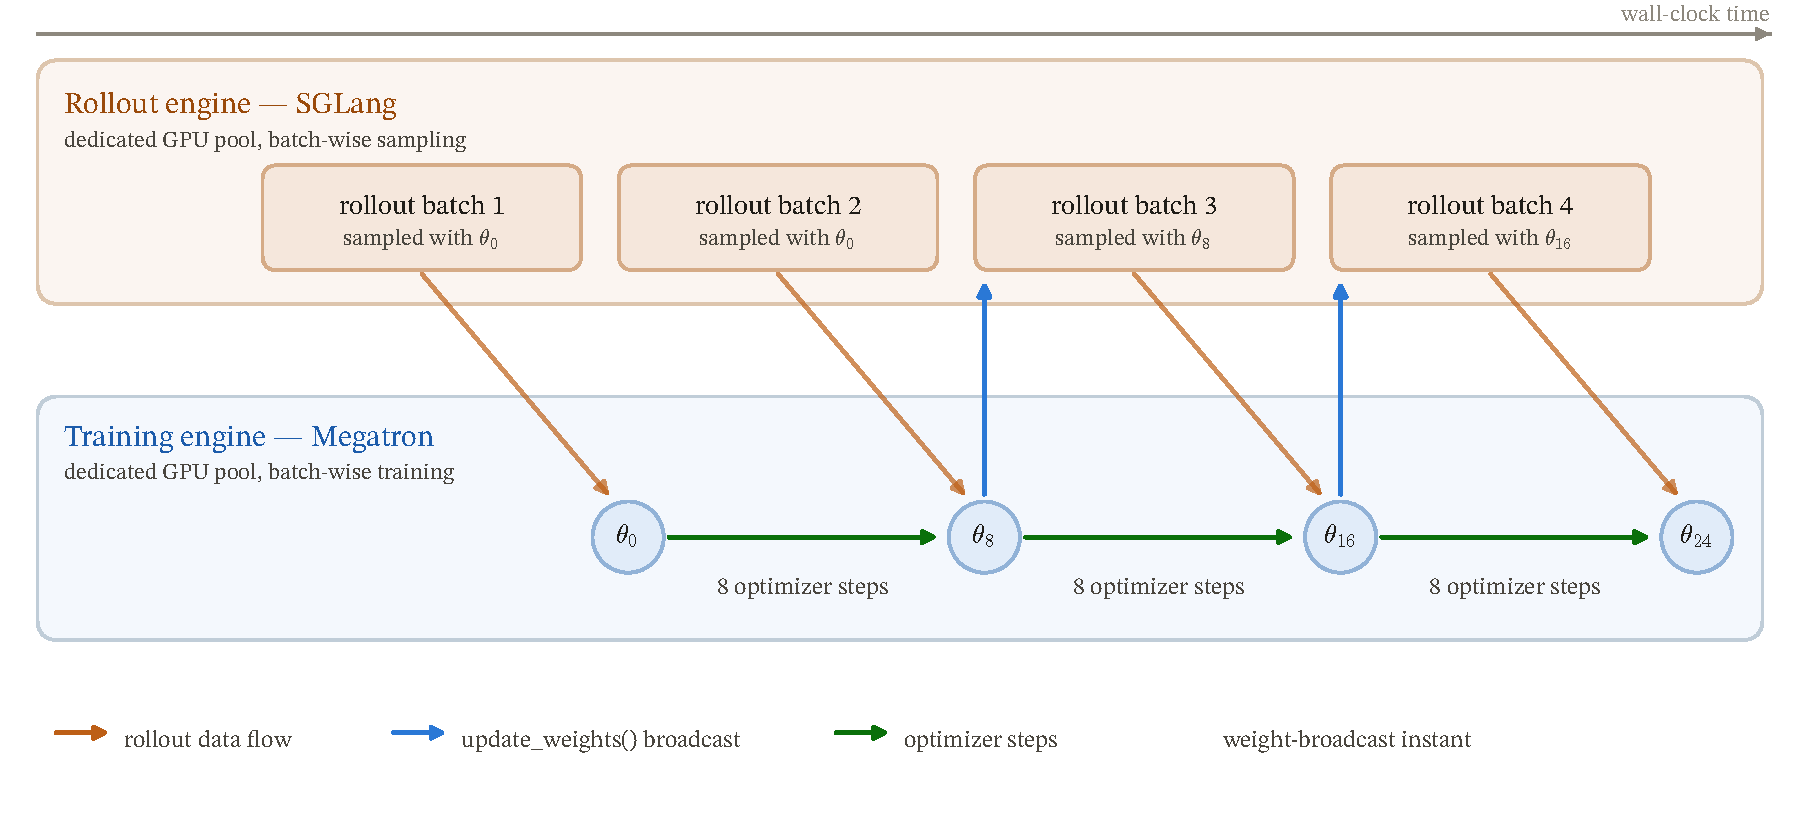
\includegraphics[width=0.85\linewidth]{figures/workflow/async_rl_pipeline.pdf}
\caption{\textbf{Batch-wise asynchronous RL.} Rollout and optimization run on decoupled resources with periodic weight broadcast, so one in-flight batch is typically trained at a configured lag of $n$ policy versions. This is the setting behind $\mu_{b,t}$, $\pi^{(j)}$, and $d_{b,t}$. 
With full notation table shown in Appendix~\ref{app:notation},
synchronous RL and fully Asynchronous RL workflows can be found in Appendix~\ref{app:sync-rl} and Appendix~\ref{app:fully-async}, respectively.}
\label{fig:pipeline}
\end{figure}

\FloatBarrier

\paragraph{Configured lag versus realized mismatch in batch-wise asynchronous RL.}
Our experiments use the batch-wise asynchronous regime of Figure~\ref{fig:pipeline}: weights are broadcast every $n$ trainer steps, and we call $n$ the \emph{configured lag}. Write $d_{b,t}=\log r_{b,t}$ for the observed sampled mismatch, let $\pi^{(\ell)}$ be the trainer-side reference log-probability at the rollout checkpoint, and define $\Delta_{b,t}^{\pi}=\log\pi^{(j)}-\log\pi^{(\ell)}$ and $\Delta_{b,t}^{\mathrm{impl}}=\log\pi^{(\ell)}-\log\mu_{b,t}$ at $(y_{b,t},s_{b,t})$. Then:
\begin{equation}
d_{b,t}
\;=\;\log r_{b,t}
\;=\;\Delta_{b,t}^{\pi}
\;+
\;\Delta_{b,t}^{\mathrm{impl}},
\label{eq:split}
\end{equation}
where $\Delta_{b,t}^{\pi}$ is the policy-update mismatch accumulated over the $n$ optimizer steps of the window and $\Delta_{b,t}^{\mathrm{impl}}$ is the implementation mismatch between the trainer-side reference and the actual rollout engine. The first term $\Delta_{b,t}^{\pi}$ is the object PPO's ratio machinery is designed to correct. 
$\Delta_{b,t}^{\mathrm{impl}}$ can remain nonzero even at identical weights because the two engines differ in kernels, numerics, and MoE routing. Engine, router, and hardware effects are useful \emph{diagnostic hypotheses} inside $\Delta_{b,t}^{\mathrm{impl}}$, but without additional intermediate distributions they do not form a unique additive decomposition; Appendix~\ref{app:sources} discusses them in that spirit. The operational consequence is the one stated in the introduction: the configured lag does not determine the realized distribution of $d_{b,t}$, so any mechanism keyed directly to $n$ addresses only part of the problem.

% \subsection{Staleness-associated training instability}
% \label{sec:bound}



% \begin{figure}[htbp]
% \centering
% \begin{subfigure}[t]{0.495\linewidth}
% \centering
% 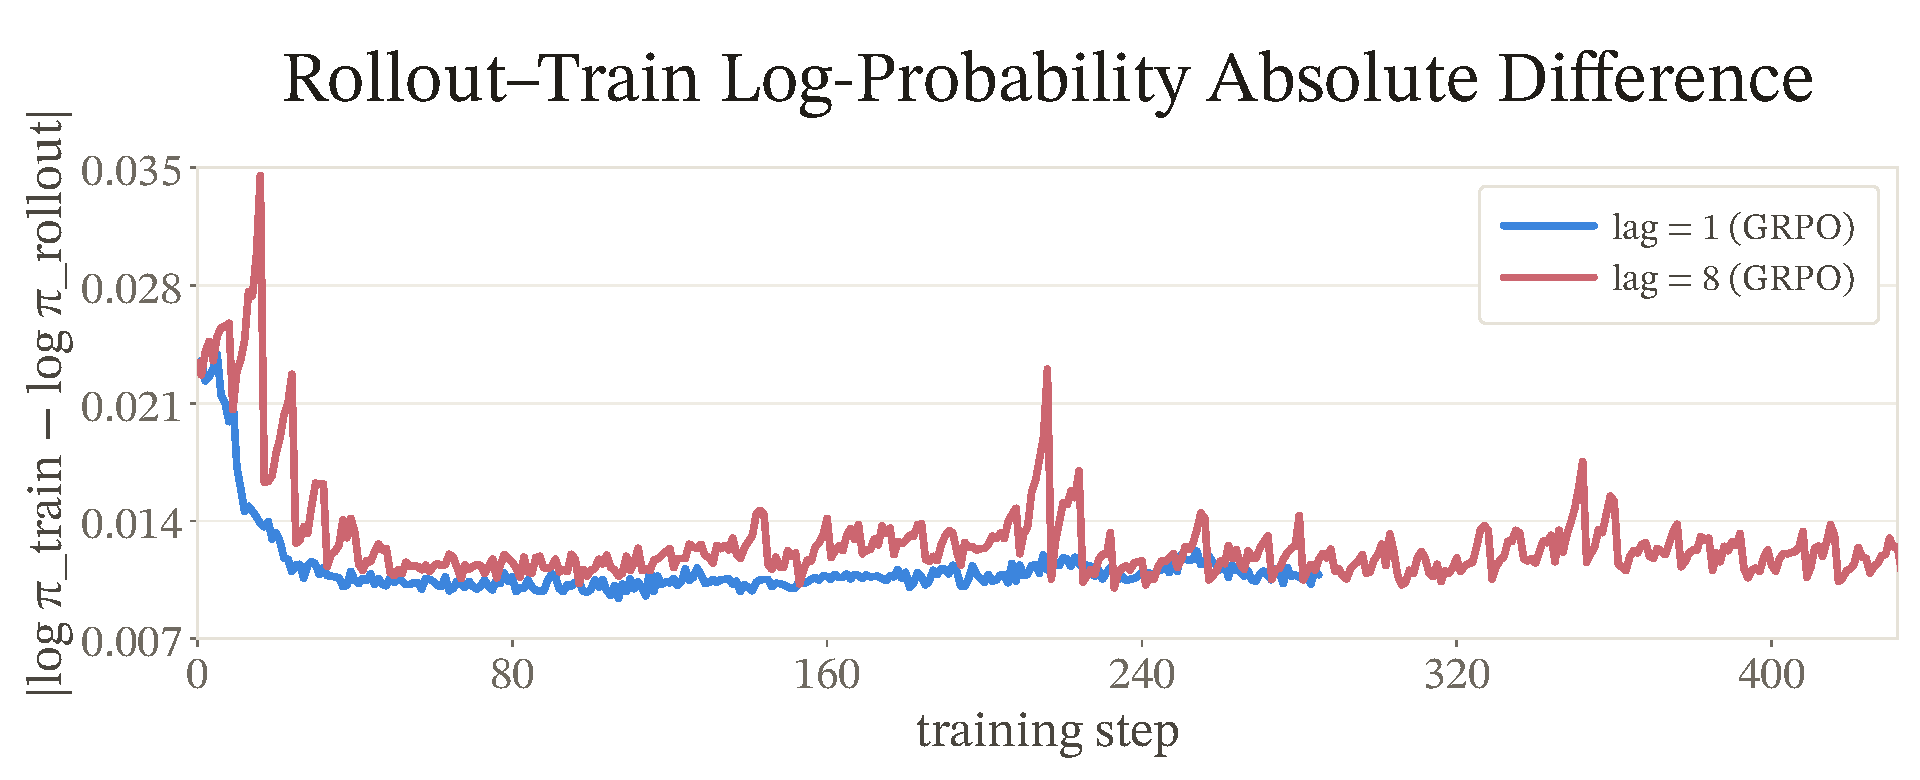
\includegraphics[width=\linewidth]{figures/charts/section_2_1_logprob_mismatch.pdf}
% \caption{Training--inference mismatch $\dpi$.}
% \label{fig:collapse-dpi}
% \end{subfigure}\hfill
% \begin{subfigure}[t]{0.495\linewidth}
% \centering
% 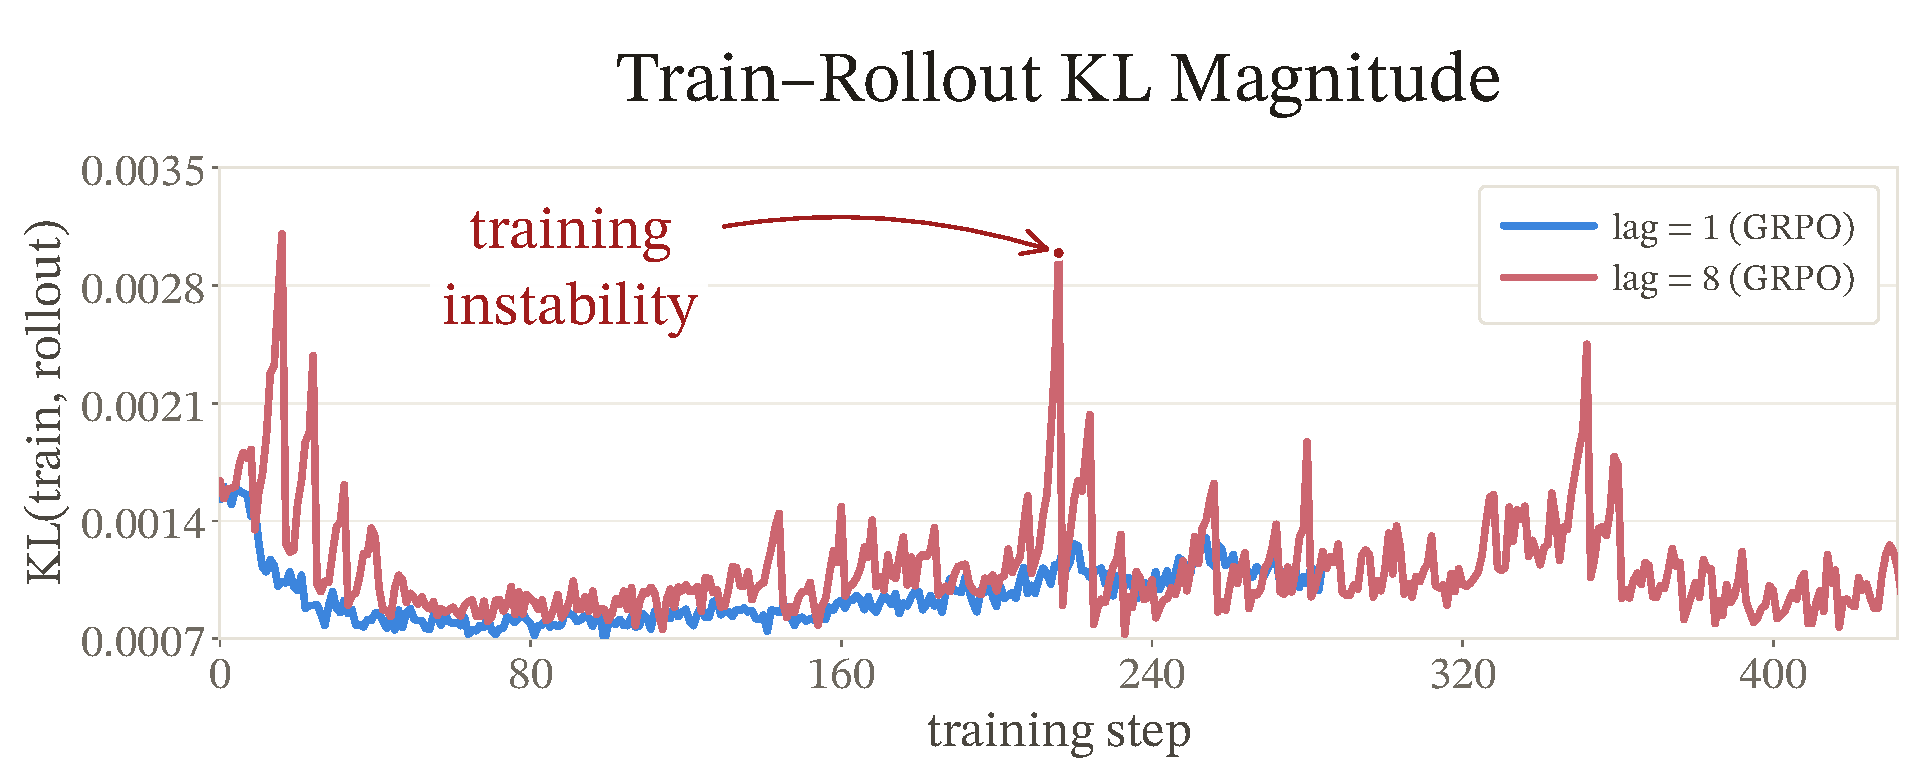
\includegraphics[width=\linewidth]{figures/charts/section_2_1_kl_magnitude.pdf}
% \caption{Train--rollout $\mathrm{KL}$.}
% \label{fig:collapse-kl}
% \end{subfigure}
% \caption{\textbf{Background instability diagnostics under GRPO at configured lag $1$ and $8$.} At lag $1$, both $\dpi$ and $|\mathrm{KL}|$ stay near their low baseline bands. At lag $8$, both rise sharply, with $\dpi$ exceeding $0.03$ and $|\mathrm{KL}|$ exceeding $2.8\times 10^{-3}$.}
% \label{fig:collapse-diagnostics}
% \end{figure}

% \begin{figure}[htbp]
% \centering
% 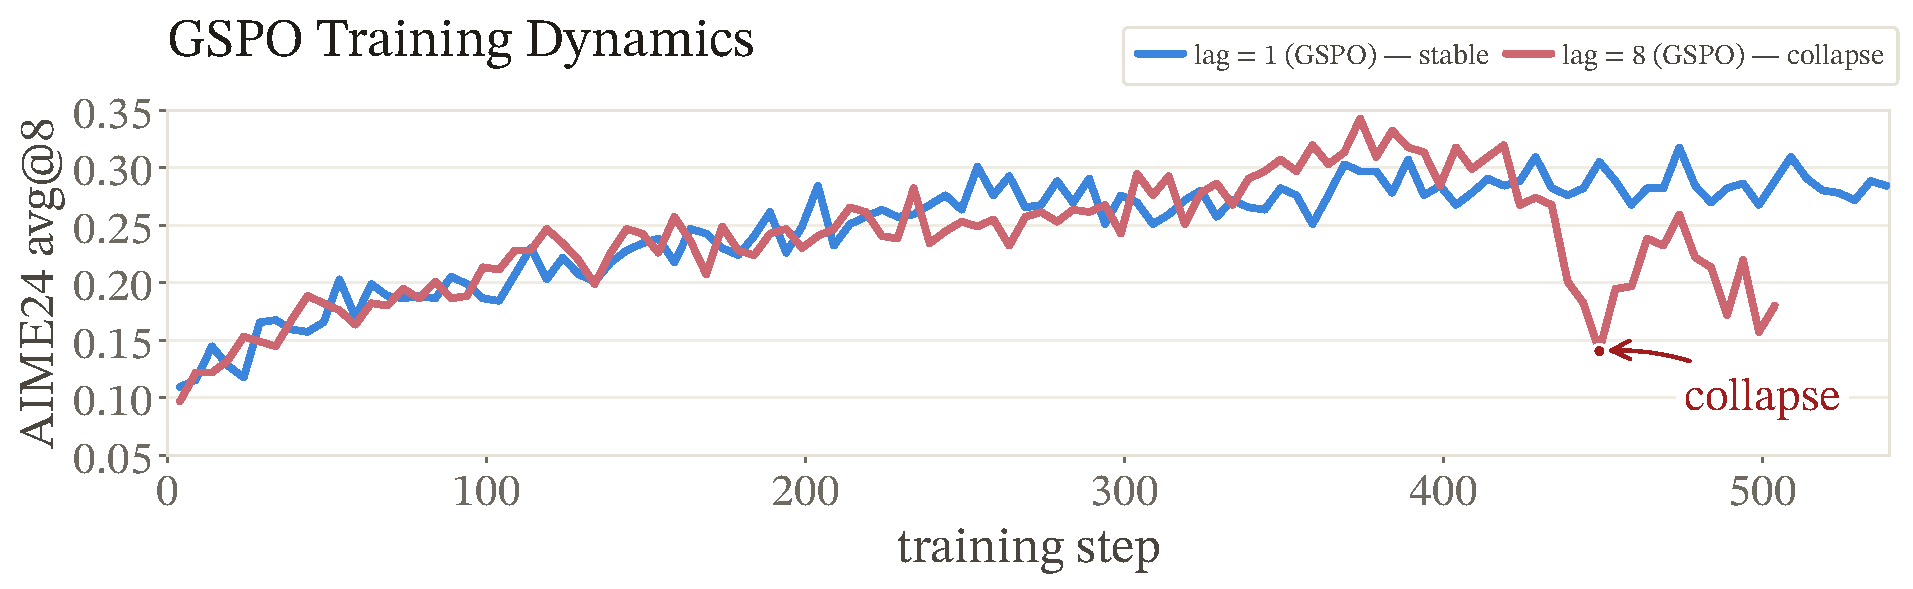
\includegraphics[width=0.85\linewidth]{figures/charts/section_2_1_aime24_pass1.pdf}
% \caption{\textbf{Background evaluation collapse under GSPO at configured lag $1$ and $8$.} The lag-$1$ run stays near the $0.30$ avg@8 band, while the lag-$8$ run peaks near $0.34$ and then falls to about $0.14$ by step $449$.}
% \label{fig:collapse-aime}
% \end{figure}

% Two symptoms recur across these batch-wise async high-lag runs, summarized by Figure~\ref{fig:collapse-diagnostics} and Figure~\ref{fig:collapse-aime}. First, \emph{mismatch inflation}: under an otherwise identical GRPO setup, the sampled mismatch $\dpi$ and its KL counterpart remain flat at configured lag $1$ but oscillate and spike at lag $8$. Second, \emph{evaluation collapse}: the lag-$8$ GSPO run reaches a few good checkpoints and then falls sharply, at a step that coincides with the mismatch leaving its earlier band. These background experiments motivate the two theory questions answered next: how LLM policy improvement should be written in the async setting, and what kind of ratio guardrail the sampled objective can actually justify.


\subsection{Staleness-associated training instability}
\label{sec:bound}

Our experiments point to a crucial background fact: once the batch-wise async lag becomes large enough, the main issue is no longer only a looser lower bound but an observable loss of training stability. In the controlled comparisons below, all runs share optimizer, data, reward, and model; only the configured lag differs. We therefore read these figures as background evidence for what async RL must explain, not as a theorem about a unique causal threshold.

\begin{figure}[htbp]
\centering
\begin{subfigure}[t]{0.495\linewidth}
\centering
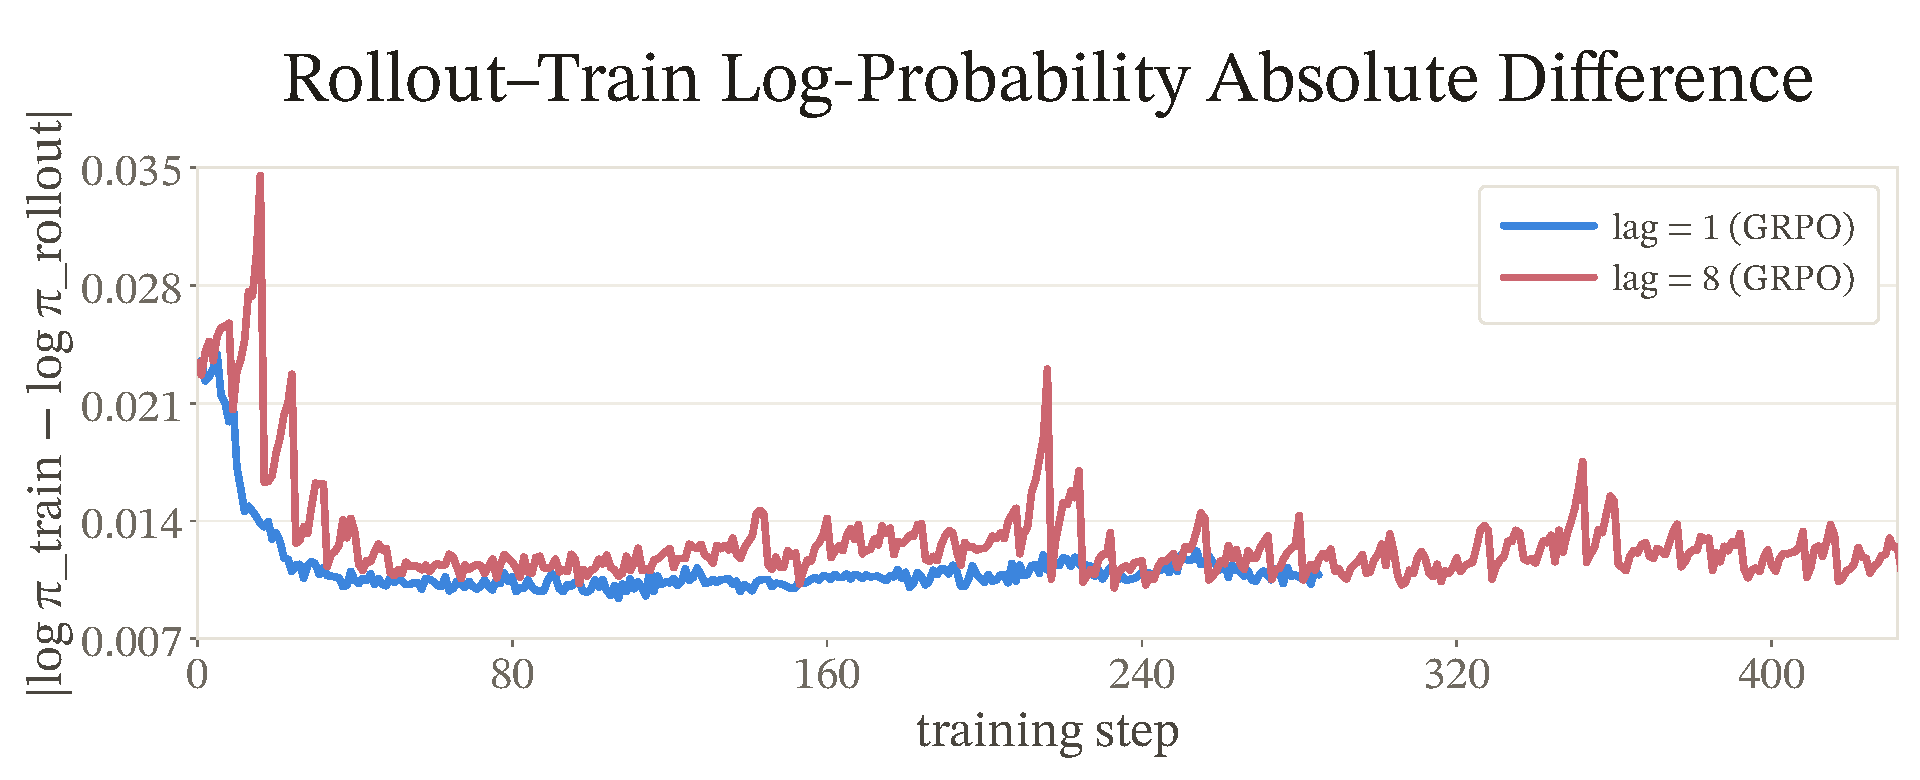
\includegraphics[width=\linewidth]{figures/charts/section_2_1_logprob_mismatch.pdf}
\caption{Training--inference mismatch $\dpi$.}
\label{fig:collapse-dpi}
\end{subfigure}\hfill
\begin{subfigure}[t]{0.495\linewidth}
\centering
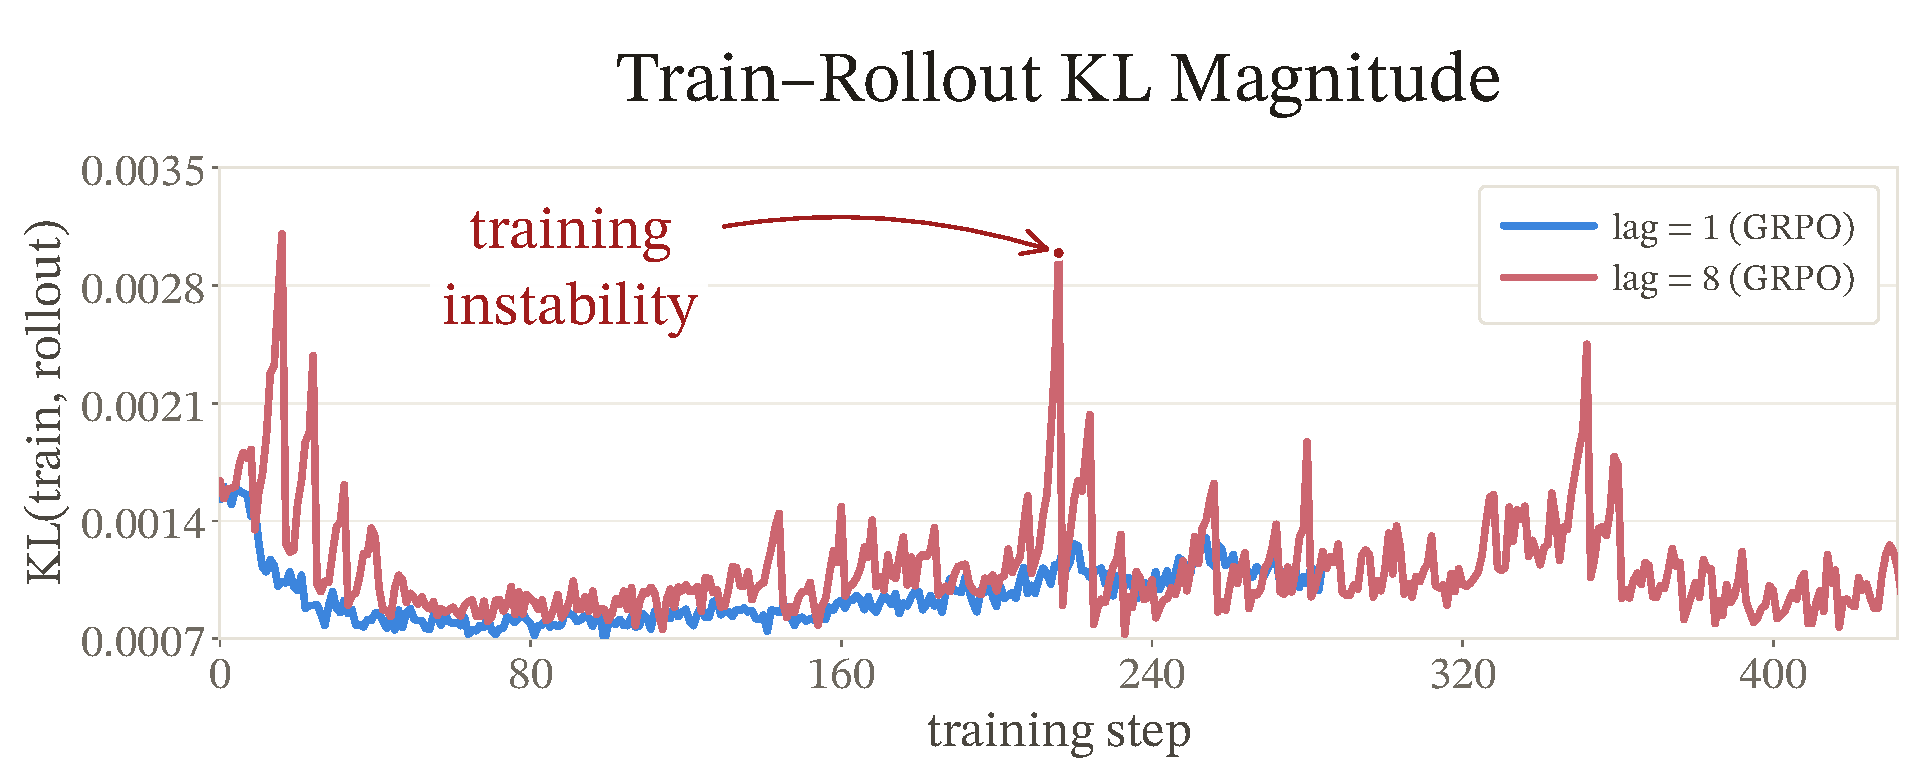
\includegraphics[width=\linewidth]{figures/charts/section_2_1_kl_magnitude.pdf}
\caption{Train--rollout $\mathrm{KL}$.}
\label{fig:collapse-kl}
\end{subfigure}
\caption{\textbf{Background instability diagnostics under a variance method at configured lag $1$ and $8$.} This figure tracks two batch-averaged mismatch diagnostics of a variance method across training under two configured lag settings, with the two curves in each panel distinguishing the mild-lag and high-lag runs under an otherwise identical setup. The panels also mark where the high-lag run first leaves its low-mismatch baseline band, together with the numerical range covered by each axis.}
\label{fig:collapse-diagnostics}
\end{figure}

\begin{figure}[htbp]
\centering
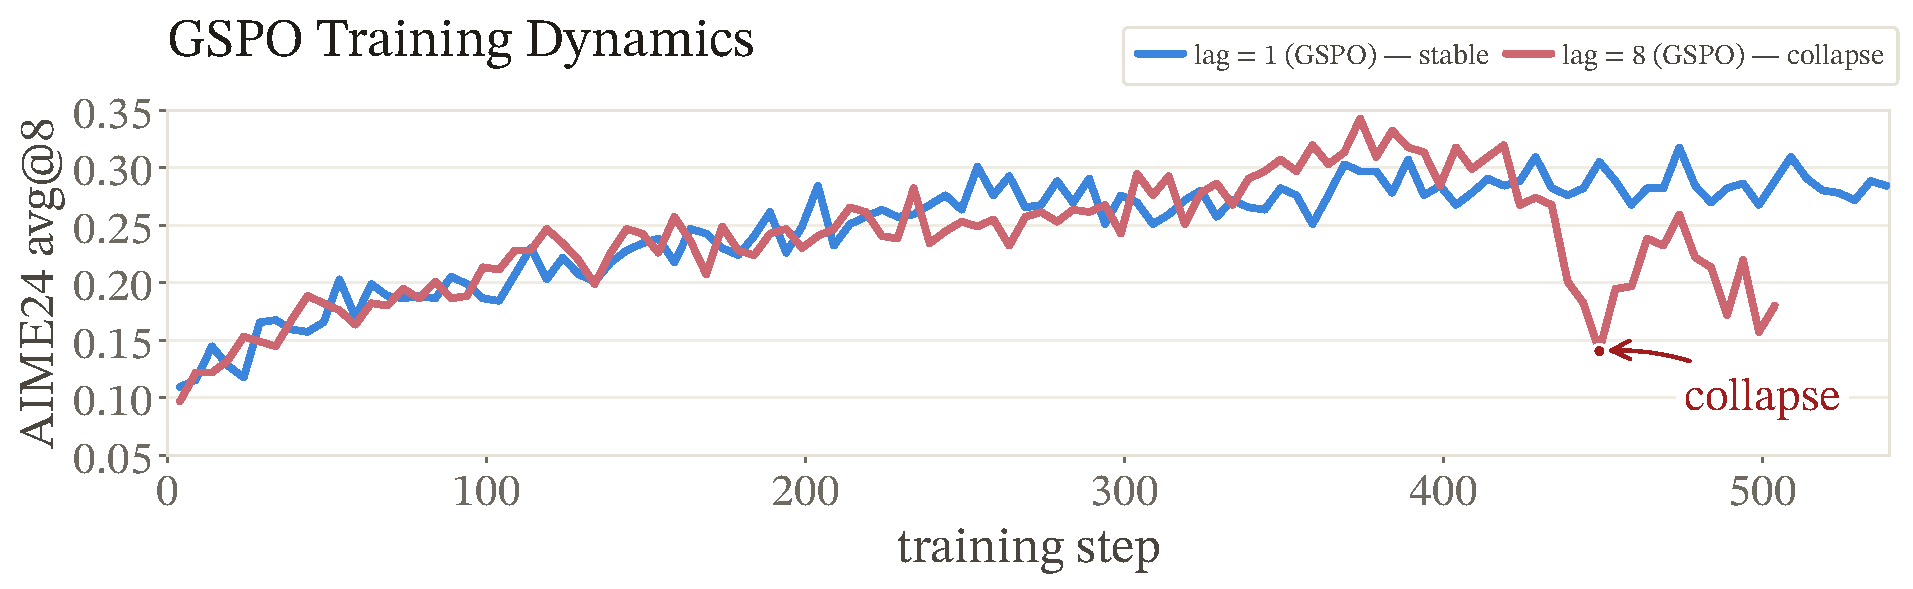
\includegraphics[width=0.85\linewidth]{figures/charts/section_2_1_aime24_pass1.pdf}
\caption{\textbf{Background evaluation collapse under a variance method at configured lag $1$ and $8$.} This figure plots the evaluation benchmark score of a variance method across training under two configured lag settings, where the collapse step of the high-lag run is explicitly annotated with a point and label. The panel is used to align the timing of evaluation collapse with the mismatch signals of Figure~\ref{fig:collapse-diagnostics}.}
\label{fig:collapse-aime}
\end{figure}

% \textbf{Two instability symptoms recur under high-lag asynchronous training.} Figure~\ref{fig:collapse-diagnostics} and Figure~\ref{fig:collapse-aime} together isolate crucial symptoms across batch-wise asynchronous runs. 
% First, \emph{mismatch inflation}: under an otherwise identical setup, the sampled mismatch $\dpi$ and its KL counterpart remain flat at configured lag $1$ but oscillate and spike at lag $8$, with $\dpi$ exceeding $0.03$ and the KL diagnostic exceeding $2.8\times 10^{-3}$. Second, \emph{evaluation collapse}: the lag-$1$ run stays near the $0.30$ evaluation-benchmark band, while the lag-$8$ run peaks near $0.34$ and then falls sharply to about $0.14$ by step $449$, at a step that coincides with the mismatch leaving its earlier band. These background experiments motivate the two theory questions answered next: how LLM policy improvement should be written in the async setting, and what kind of ratio guardrail the sampled objective can actually justify.

\textbf{Two instability symptoms recur under high-lag asynchronous training.} Figure~\ref{fig:collapse-diagnostics} and Figure~\ref{fig:collapse-aime} shows how batch-wise asynchronous training deteriorate as the lag grows, from which three observations stand out.
\begin{itemize}
    \item \textbf{Mismatch inflation under increased staleness.} Mismatch $\dpi$ and its KL counterpart stay in a narrow band at lag $1$ but develop heavy-tailed spikes at lag $8$, where $\dpi$ exceeds $0.03$ and the KL diagnostic exceeds $2.8\times 10^{-3}$, indicating a widening of the ratio distribution rather than a shift of its center.
    \item \textbf{Training collapse due to increase of staleness.} The lag-$1$ run tracks the evaluation-benchmark band near $0.30$, whereas the lag-$8$ run peaks near $0.34$ before falling to about $0.14$ by step $449$. 
    % The decline coincides with the mismatch signal leaving its stationary band, suggesting a delayed downstream response to ratio drift.
    % \item \textbf{Two theoretical questions raised by these diagnostics.} These trajectories motivate the remainder of the paper: how the LLM policy improvement objective should be expressed under train--rollout divergence, and what ratio guardrail the sampled surrogate can justify when the induced drift is heavy-tailed.
\end{itemize}

% =====================================================================
% 3 LLM policy improvement in async RL
% =====================================================================
\section{LLM Policy Improvement and Ratio Control in Async RL}
\label{sec:ppo-soft}

\subsection{Finite-horizon LLM policy-improvement surrogate}
\label{sec:llm-pi}

Consider an undiscounted, finite-horizon generation problem with $|R(y)|\le\xi$, behavior policy $\mu$, and target policy $\pi$, and define $\J(\pi)=\E_{y\sim\pi}[R(y)]$. We assume trajectory support compatibility: at every $\mu$-reachable state used below, $\pi(\cdot\mid s)\ll\mu(\cdot\mid s)$. When necessary, an end-of-sequence action and padding make the horizon fixed. Following the Kakade--Langford line of analysis~\citep{kakade2002approximately,schulman2015trpo}, define the linear surrogate:
\begin{equation}
L'_{\mu}(\pi)\;=\;\E_{y\sim\mu}\!\left[R(y)\sum_{t=1}^{T}\Big(\frac{\pi(y_t\mid s_t)}{\mu(y_t\mid s_t)}-1\Big)\right].
\label{eq:surrogate}
\end{equation}
A representative finite-horizon lower bound~\citep{qi2026dppo} is:
\begin{equation}
\J(\pi)-\J(\mu)\;\geq\;L'_{\mu}(\pi)\;-
4\xi\,\E_{y\sim\mu}\!\left[\sum_{t=1}^{T}\dtv\big(\mu(\cdot\mid s_t)\,\|\,\pi(\cdot\mid s_t)\big)\right].
\label{eq:tvbound}
\end{equation}
The penalty is an expected \emph{cumulative} token-level divergence, not a length-normalized average. Equation~\eqref{eq:tvbound} is the policy-improvement statement relevant for the rest of the paper: smaller statewise divergence makes the approximation term less pessimistic, but it does not by itself imply that an arbitrary smaller update is automatically better. Non-decrease still depends on the surrogate gain dominating the divergence penalty.

% In a genuinely asynchronous system the behavior conditional can vary with the realized scheduler and policy version. Equation~\eqref{eq:tvbound} should then be read conditional on that schedule, or after augmenting the state with the relevant scheduler/version information so that the trajectory behavior factorizes through the stated conditionals.

\subsection{Ratio envelopes and the sampled clip in async RL}
\label{sec:ratio-envelope}

The relation between ratio control and Section~\ref{sec:llm-pi}'s policy-improvement surrogate is exact but conditional on support compatibility.

\begin{lemma}[\textbf{Ratio deviation as a statewise divergence identity}]
\label{lem:tv-ratio}
Fix a state $s$ and suppose $\pi(\cdot\mid s)\ll\mu(\cdot\mid s)$. Then, with $r_s(a)=\pi(a\mid s)/\mu(a\mid s)$,
\begin{equation}
\dtv\big(\mu(\cdot\mid s)\,\|\,\pi(\cdot\mid s)\big)
\;=\;\frac12\,\E_{a\sim\mu(\cdot\mid s)}\big|r_s(a)-1\big|.
\label{eq:tvid}
\end{equation}
\end{lemma}
% \begin{myproof}
\textbf{Proof.}
$\frac12\sum_{a}|\pi(a\mid s)-\mu(a\mid s)|=\frac12\sum_{a}\mu(a\mid s)\,|r_s(a)-1|$; absolute continuity rules out unaccounted target mass on actions with $\mu(a\mid s)=0$.
% \end{myproof}

% Full-vocabulary softmax sampling satisfies the support condition in exact arithmetic---our experiments disable nucleus truncation for precisely this reason (Section~\ref{sec:exp-setup}). Top-$k$ or top-$p$ truncation can violate it and requires separate treatment (Appendix~\ref{app:stabilizers}).
Full-vocabulary softmax sampling satisfies the support condition in exact arithmetic, which is why our experiments in Section~\ref{sec:exp-setup} disable nucleus truncation. However, top-$k$ or top-$p$ truncation can violate this condition and requires the separate treatment discussed in Appendix~\ref{app:stabilizers}.

Equation~\eqref{eq:tvid} is the step that connects a hard ratio envelope to the policy-improvement bound of Equation~\eqref{eq:tvbound}. If, at a fixed state, every action satisfies a hard ratio bound, then the divergence term in Equation~\eqref{eq:tvbound} is correspondingly controlled:
\begin{proposition}[\textbf{Ideal all-action ratio region}]
\label{prop:hard-ratio}
Under the conditions of Lemma~\ref{lem:tv-ratio}, if:
\begin{equation}
|r_s(a)-1|\;\le\;\varepsilon\qquad\text{for $\mu$-almost every action $a$,}
\label{eq:all-action}
\end{equation}
then $\dtv(\mu\,\|\,\pi)[s]\le\varepsilon/2$. More generally, if $1-\varepsilon_{\mathrm{low}}(a)\le r_s(a)\le 1+\varepsilon_{\mathrm{high}}(a)$ for every action, then:
\begin{equation}
\dtv(\mu\,\|\,\pi)[s]\;\le\;\frac12\,\E_{a\sim\mu}\max\big\{\varepsilon_{\mathrm{low}}(a),\,\varepsilon_{\mathrm{high}}(a)\big\},
\label{eq:asym-tv}
\end{equation}
which for constant asymmetric radii is at most $\tfrac12\max\{\elow,\ehigh\}$.
\end{proposition}
\textbf{Proof.}
Each assumption gives the corresponding pointwise bound on $|r_s(a)-1|$, substitution into Equation~\eqref{eq:tvid} proves each claim.
% \end{myproof}

This proposition describes an \emph{ideal all-action feasible set}. The quantifier is essential: a bound on the one sampled action says nothing about the rest of the vocabulary distribution. That gap is exactly why sampled clipping in async RL should be read as a surrogate motivated by the hard-envelope argument above, not as the hard envelope itself.

% For a sampled token $(b,t)$ with ratio $r_{b,t}$ as in Equation~\eqref{eq:ratio-def} and advantage $\hat A_{b,t}$, the PPO sampled surrogate with possibly asymmetric radii is:
% \begin{equation}
% \mathcal S^{\mathrm{PPO}}_{b,t}
% =\min\!\Big(r_{b,t}\hat A_{b,t},\;\bar r^{\mathrm{PPO}}_{b,t}\hat A_{b,t}\Big),
% \qquad
% \bar r^{\mathrm{PPO}}_{b,t}=\clip\!\big(r_{b,t},\,1-\elow,\,1+\ehigh\big),
% \label{eq:ppo-objective}
% \end{equation}
% and the loss minimized in code is $-\mathcal S^{\mathrm{PPO}}_{b,t}$.

% Equation~\eqref{eq:ppo-objective} does not enforce $|r_{b,t}-1|\le\varepsilon$, even for the sampled token. It changes the objective branch; it neither projects the learned policy into a ratio interval nor inspects any unobserved action. The advantage sign creates a useful asymmetry:
% \begin{table}[h]
% \centering
% \small
% \begin{tabularx}{0.92\textwidth}{@{}lllX@{}}
% \toprule
% Advantage & Ratio region & PPO branch & Local update interpretation \\
% \midrule
% $\hat A>0$ & $r>1+\ehigh$ & clipped & outward increase is stopped \\
% $\hat A>0$ & $r<1-\elow$ & unclipped & gradient increases $r$ toward one (pull-back) \\
% $\hat A<0$ & $r<1-\elow$ & clipped & outward decrease is stopped \\
% $\hat A<0$ & $r>1+\ehigh$ & unclipped & gradient decreases $r$ toward one (pull-back) \\
% \bottomrule
% \end{tabularx}
% \end{table}

% \paragraph{Metrics and statistical scope.}The clipped branch is flat only when the advantage would push the ratio \emph{farther} from one; whenever the update direction pulls the sampled ratio back toward one, the gradient is deliberately retained, however large $|r-1|$ already is. In this paper, that is the precise relation between ratio control and policy improvement in async RL: the hard all-action envelope would control the divergence term in Equation~\eqref{eq:tvbound}, while PPO clipping only supplies a sampled, soft guardrail motivated by that argument. Every claim we make about \satr{} lives at this same surrogate level.

% =====================================================================
% 4 SATR
% =====================================================================
\section{\satr: From Heterogeneous Mismatch to an Adaptive Clip}
\label{sec:satr}

% \subsection{Why a fixed radius is an imperfect default}
% \label{sec:satr-motivation}

% A fixed $\varepsilon$ treats every sampled token as equally reliable. In an asynchronous pipeline, however, the realized mismatch is heterogeneous: most tokens remain close to the behavior policy while a small tail is affected by policy lag, training--inference engine differences, router choices, or numerical effects. Setting a uniformly tiny radius suppresses useful learning on the bulk of the data; setting a uniformly large radius leaves the high-staleness tail with the same outward allowance as reliable tokens.

% \satr{} uses the sampled log-ratio to adapt the \emph{nominal} radius. The method does not interpret $|\log r|$ as $D_{\mathrm{TV}}$. Indeed, the sampled action's contribution to the $D_{\mathrm{TV}}$ sum carries a behavior-probability weight:
% \begin{equation}
% \tfrac12\,\mu(a\mid s)\,\big|r(a\mid s)-1\big|\;=\;\tfrac12\,\big|\pi(a\mid s)-\mu(a\mid s)\big|,
% \label{eq:tv-mass}
% \end{equation}
% so a rare action can have an enormous ratio while moving little probability mass. The log-ratio is used because it is already observable in off-policy training and empirically exposes the long mismatch tail; its suitability as the risk score is an empirical design choice, and probability-mass-weighted alternatives are natural follow-ups (Section~\ref{sec:limitations}).
\subsection{From Policy Improvement to a Staleness-Adaptive Radius}
\label{sec:satr-motivation}
Section~\ref{sec:ppo-soft} ends one step short of a method: shown in Lemma~\ref{lem:tv-ratio}, statewise divergence controls the finite-horizon approximation term, that divergence is exactly a behavior expectation of absolute ratio deviation, and a hard all-action ratio envelope would therefore control the penalty, as discussed in Proposition~\ref{prop:hard-ratio}, but nothing yet says what the \emph{sampled} objective should do when the envelope is unavailable. To make the target of that chain explicit, we name once the two LLM-regime divergence quantities:
\begin{equation}
\begin{gathered}
D_{\mathrm{TV}}^{\max}(\mu\|\pi)\triangleq \max_{s_t} D_{\mathrm{TV}}\bigl(\mu(\cdot\mid s_t)\|\pi(\cdot\mid s_t)\bigr),\\
D_{\mathrm{TV}}(\mu,\pi)\triangleq \mathbb{E}_{y\sim\mu}\!\left[\sum_{t=1}^{|y|} D_{\mathrm{TV}}\bigl(\mu(\cdot\mid s_t)\|\pi(\cdot\mid s_t)\bigr)\right].
\end{gathered}
\label{eq:satr-divergences}
\end{equation}
In finite-horizon LLM setting with horizon $T$, $\gamma=1$, and $\xi=\max_y |R(y)|$, the improvement gap admits both:
\begin{align}
\J(\pi)-\J(\mu)
&\ge L'_{\mu}(\pi)-2\xi\,T(T-1)\,\bigl(D_{\mathrm{TV}}^{\max}(\mu\|\pi)\bigr)^{2},\label{eq:satr-maxbound}\\
\J(\pi)-\J(\mu)
&\ge L'_{\mu}(\pi)-4\xi\,D_{\mathrm{TV}}(\mu,\pi).
\label{eq:satr-avgbound}
\end{align}
The first is the finite-horizon analogue of a max-divergence trust-region bound; the second restates Equation~\eqref{eq:tvbound} in the named notation and is the cumulative token-level form that a token-wise sampled objective can actually influence on long responses. What PPO optimizes, however, is neither bound but the sampled clipped surrogate:
\begin{equation}
\mathcal S^{\mathrm{PPO}}_{b,t}
=\min\!\Big(r_{b,t}\hat A_{b,t},\;\bar r^{\mathrm{PPO}}_{b,t}\hat A_{b,t}\Big),
\qquad
\bar r^{\mathrm{PPO}}_{b,t}=\clip\!\big(r_{b,t},\,1-\elow,\,1+\ehigh\big),
\label{eq:ppo-objective}
\end{equation}
whose only guardrail is the fixed pair $(\elow,\ehigh)$: the clipped branch suppresses outward gradients beyond the nominal boundary, preserves pull-back updates, and inspects nothing beyond the one sampled action.
 
\paragraph{Why a fixed radius is an imperfect default.}
A fixed $\varepsilon$ treats every sampled token as equally reliable. In the batch-wise asynchronous pipeline of Section~\ref{sec:tv}, however, the realized mismatch $d_{b,t}$ mixes policy-update and implementation terms in Equation~\eqref{eq:split} and is heterogeneous within a single rollout window: most tokens remain close to the behavior policy, while a small tail is affected by policy lag, training--inference engine differences, router choices, or numerical effects. A uniformly tiny radius therefore suppresses useful learning on the bulk of the data, while a uniformly large radius grants the high-staleness tail the same outward allowance as reliable tokens. Read against Equations~\eqref{eq:satr-maxbound}--\eqref{eq:satr-avgbound}, both defaults miss the point: the divergence penalty is driven by where the mismatch is large, and no single global radius can be simultaneously permissive on the bulk and conservative on the tail.

\paragraph{A sampled proxy, not a divergence estimate.}
The observable that exposes this tail is the sampled log-ratio $d_{b,t}=\log r_{b,t}$, which is already computed in off-policy training. It must not, however, be interpreted as $D_{\mathrm{TV}}$: the sampled action's contribution to the $D_{\mathrm{TV}}$ sum carries a behavior-probability weight,
\begin{equation}
\tfrac12\,\mu(a\mid s)\,\big|r(a\mid s)-1\big|\;=\;\tfrac12\,\big|\pi(a\mid s)-\mu(a\mid s)\big|,
\label{eq:tv-mass}
\end{equation}
so a rare action can have an enormous ratio while moving little probability mass. As detailed in Section~\ref{sec:limitations}, its use as a per-token risk score is an empirical design choice.

\paragraph{Design of SAT.}
% \textbf{These observations fix what an adaptive rule may claim and how it should act. }It cannot impose a hard all-action trust region, so it must operate at the same surrogate level as Equation~\eqref{eq:ppo-objective}. 
These observations govern how an adaptive clipping rule should operate. Because training only observes sampled actions rather than the full distribution, the rule cannot enforce a strict, all-action trust region; instead, it must function at the same surrogate objective level as Equation~\eqref{eq:ppo-objective}.
Specifically, SAT contracts PPO's nominal interval only on tokens whose observed mismatch is unusually large {for the current batch}, and only on the side that moves the sampled ratio farther from one, with the direction that locally enlarges the divergence penalty. Consequently, it leaves ordinary tokens and pull-back updates untouched, reducing exactly to the baseline objective when disabled.

\subsection{Staleness-Adaptive Trust Region}
\label{sec:satr-method}



\textbf{{SAT targets a simple but useful goal, which reshapes the sampled PPO surrogate so that tokens with unusually large observed mismatch receive a tighter outward allowance, while ordinary tokens and pull-back updates retain the baseline behavior}}. The whole method is defined by the sequence of formulas below.

\textbf{Detached sampled token-level staleness.} \satr{} begins from the sampled mismatch signal already available in asynchronous training and treats the detached token-level log-ratio as a practical staleness proxy for the current sample:
\begin{equation}
d_{b,t}=\log r_{b,t},\qquad d^{\mathrm{sg}}_{b,t}\triangleq\sg[d_{b,t}],
\label{eq:satr-d}
\end{equation}
where $\sg$ denotes stop-gradient. This detached score is not itself optimized; it only decides how conservative the clip interval should be on the current sample.

\textbf{Staleness-based kernel function scaling.} Rather than compare $|d_{b,t}|$ with a fixed global threshold, \satr{} calibrates the high-staleness tail relative to the current batch through the detached empirical quantile:
\begin{equation}
\widehat F_{|d|}(x)=\frac{1}{|\mathcal T_{\mathrm{act}}|}\sum_{(b,t)\in\mathcal T_{\mathrm{act}}}\mathbf 1\{|d_{b,t}|\le x\},
\qquad
q=\sg\Big[\inf\{x\ge 0:\widehat F_{|d|}(x)\ge \alpha\}\Big].
\label{eq:quantile}
\end{equation}
The role of $q$ is purely referential: it marks where the current batch begins to enter its mismatch tail, where $\alpha$ denotes the target quantile threshold, which set to 0.90 in our implementation. Because $q$ is recomputed from the same active tokens being optimized, the method adapts to rescaling of the mismatch profile without introducing another hand-tuned absolute cutoff.
\satr{} then maps the sign-separated mismatch magnitudes through a monotone kernel:
\begin{equation}
\psi(u;q)=\frac{1}{1+(u/q)^{2}},
\qquad
u_{+,b,t}=\pos{d^{\mathrm{sg}}_{b,t}},\quad u_{-,b,t}=\pos{-d^{\mathrm{sg}}_{b,t}},
\label{eq:kernel}
\end{equation}
where $\psi(0;q)=1$, $\psi(q;q)=\tfrac12$, and $\partial\psi/\partial u\le 0$. The sign split is the key structural choice: when the sampled ratio is already above $1$, the adaptive rule should only tighten the upper side of the interval; when it is below $1$, it should only tighten the lower side. Otherwise the method would also suppress pull-back moves that already head back toward the behavior policy.

\textbf{Effective contraction factors.} The contraction is applied only on the high-staleness tail:
\begin{equation}
c_{\pm,b,t}=
\begin{cases}
\psi(u_{\pm,b,t};q), & q>0\ \text{and}\ |d^{\mathrm{sg}}_{b,t}|>q,\\[2pt]
1, & \text{otherwise},
\end{cases}
\label{eq:gate}
\end{equation}
which yields the adaptive radii:
\begin{equation}
\tilde\varepsilon_{\mathrm{low},b,t}=\elow\,c_{-,b,t},
\qquad
\tilde\varepsilon_{\mathrm{high},b,t}=\ehigh\,c_{+,b,t}.
\label{eq:adaptive-eps}
\end{equation}
Since $0<c_{\pm,b,t}\le 1$, these radii never expand the original PPO interval. Ungated tokens recover the baseline radii exactly, while gated positive-mismatch tokens only shrink the upper side and gated negative-mismatch tokens only shrink the lower side.
\begin{itemize}
\item \textbf{SAT core mechanism.} \satr{} is conservative only where the sampled mismatch is unusually large and only on the side that would move the sampled ratio farther away from one. The explicit $q>0$ branch avoids division by zero when most mismatch values vanish, and under the inverse-cumulative distribution function convention the strict gate $|d|>q$ selects at most the top decile of active positions.
\end{itemize}

\textbf{SAT sampled objective.} \satr{} then obtains the final sampled surrogate by dropping the adaptive radii into the original clipped objective:
\begin{align}
\bar r^{\satr}_{b,t}&=\clip\!\big(r_{b,t},\,1-\tilde\varepsilon_{\mathrm{low},b,t},\,1+\tilde\varepsilon_{\mathrm{high},b,t}\big),
\label{eq:satr-clip}\\
\mathcal S^{\satr}_{b,t}&=\min\!\big(r_{b,t}\hat A_{b,t},\;\bar r^{\satr}_{b,t}\hat A_{b,t}\big).
\label{eq:satrloss}
\end{align}
This substitution shows that \satr{} is not a new objective family but a drop-in replacement for PPO clipping: it replaces $\bar r^{\mathrm{PPO}}_{b,t}$ by $\bar r^{\satr}_{b,t}$ inside the same sampled surrogate. When $c_{\pm,b,t}=1$, the underlying base objective is recovered exactly. Because the sign-selected endpoint moves inward, the adaptive interval remains contained in PPO's nominal interval, while the untouched side matches PPO. Pull-back branches therefore stay unchanged, and only the outward band between the adaptive and nominal boundaries is newly clipped.
% The extra cost is one quantile plus a few elementwise tensor operations per batch.

\paragraph{Sequence-level objectives.}
Equations~\eqref{eq:satr-d}--\eqref{eq:satrloss} describe the token-ratio implementation. For the reported GSPO extension, the scalar in the clipped objective and in the \satr{} score is instead the length-normalized sequence ratio:
\begin{equation}
\rho^{\mathrm{seq}}_{b}=\exp\!\Big(\frac{1}{T_b}\sum_{t=1}^{T_b}\log r^{\mathrm{tok}}_{b,t}\Big),
\qquad
r^{\mathrm{tok}}_{b,t}=\frac{\pi^{(j)}(y_{b,t}\mid s_{b,t})}{\mu_{b,t}(y_{b,t}\mid s_{b,t})},
\label{eq:gspo-ratio}
\end{equation}
broadcast to the response's active token positions before the same active-token quantile and objective aggregation are applied. The empirical quantile therefore length-weights sequences, and every token of one response receives the same sequence-ratio score. 
% The interval and scalar-surrogate claims below apply verbatim after this substitution; the token-level $D_{\mathrm{TV}}$ interpretation does not, because token log-ratios can cancel inside $\rho^{\mathrm{seq}}_b$.

% \subsection{SAT reshapes update geometry from staleness-adptive}
% \label{sec:satr-mechanism}

% Following the Finite-horizon LLM policy-improvement surrogate in Section \ref{sec:llm-pi}, to place the local clip geometry in the finite-horizon improvement picture, it is useful to name once the two LLM-regime divergence quantities:
% \begin{equation}
% \begin{gathered}
% D_{\mathrm{TV}}^{\max}(\mu\|\pi)\triangleq \max_{s_t} D_{\mathrm{TV}}\bigl(\mu(\cdot\mid s_t)\|\pi(\cdot\mid s_t)\bigr),\\
% D_{\mathrm{TV}}(\mu,\pi)\triangleq \mathbb{E}_{y\sim\mu}\!\left[\sum_{t=1}^{|y|} D_{\mathrm{TV}}\bigl(\mu(\cdot\mid s_t)\|\pi(\cdot\mid s_t)\bigr)\right].
% \end{gathered}
% \label{eq:satr-divergences}
% \end{equation}
% In the finite-horizon LLM setting with horizon $T$, $\gamma=1$, and $\xi=\max_y |R(y)|$, the improvement gap admits both
% \begin{align}
% \J(\pi)-\J(\mu)
% &\ge L'_{\mu}(\pi)-2\xi T(T-1)\Bigl(\max_{s_t} D_{\mathrm{TV}}\bigl(\mu(\cdot\mid s_t)\|\pi(\cdot\mid s_t)\bigr)\Bigr)^2,\label{eq:satr-maxbound}\\
% \J(\pi)-\J(\mu)
% &\ge L'_{\mu}(\pi)-4\xi\,\mathbb{E}_{y\sim\mu}\!\left[\sum_{t=1}^{|y|} D_{\mathrm{TV}}\bigl(\mu(\cdot\mid s_t)\|\pi(\cdot\mid s_t)\bigr)\right].
% \label{eq:satr-avgbound}
% \end{align}
% The first is the finite-horizon analogue of a max-divergence trust-region bound, whereas the second is closer to the cumulative token-level control that PPO-style methods can influence on long responses. The propositions below therefore isolate only the local sampled-surrogate part of this story: \textbf{\satr{} does not impose a hard all-action trust region, but it contracts PPO's nominal interval in the direction that would locally reduce the divergence penalty. }Proposition~\ref{prop:containment} begins with that interval geometry, and Proposition~\ref{prop:pessimism} then identifies the additional outward bands that \satr{} clips.

% \begin{proposition}[Nominal interval containment]
% \label{prop:containment}
% For positive base radii, define
% $\I^{\mathrm{PPO}}=[1-\elow,\,1+\ehigh]$ and
% $\I^{\satr}_{b,t}=[1-\elow c_{-,b,t},\,1+\ehigh c_{+,b,t}]$.
% Then $\I^{\satr}_{b,t}\subseteq\I^{\mathrm{PPO}}$ for every sampled token. The intervals are equal when the gate is off; when it fires, the endpoint selected by $\operatorname{sign}(d_{b,t})$ moves strictly inward while the opposite endpoint is unchanged.
% \end{proposition}
% \textbf{x5jProof.}
% % \begin{myproof}
% Equation~\eqref{eq:gate} gives $0<c_{\pm,b,t}\le 1$. Multiplying a positive base radius by such a factor can only move the selected boundary toward $1$ or leave it fixed, so the adaptive interval is contained in PPO's interval. Strictness on the gated side follows from $\psi(u;q)<1$ at $u>q>0$.
% % \end{myproof}

% \begin{proposition}[Pointwise pessimism and newly clipped bands]
% \label{prop:pessimism}
% For the same sampled ratio $r$ and advantage $\hat A$:
% \begin{equation}
% \mathcal S^{\satr}(r,\hat A)\;\le\;\mathcal S^{\mathrm{PPO}}(r,\hat A).
% \label{eq:pessimism}
% \end{equation}
% Holding the stopped clip limits fixed and away from the clipping kinks, the derivatives with respect to $r$ differ only on the newly clipped outward bands:
% \begin{equation}
% \{\hat A>0,\ 1+\ehigh c_{+,b,t}<r<1+\ehigh\}
% \;\vee\;
% \{\hat A<0,\ 1-\elow<r<1-\elow c_{-,b,t}\}.
% \label{eq:bands}
% \end{equation}
% On those bands \satr{} has zero derivative while PPO retains its outward derivative $\hat A$. Pull-back branches are unchanged, and ratios already outward-clipped by PPO have zero derivative under both objectives.
% \end{proposition}

% \textbf{Proof.}
% For $\hat A>0$, we compare $\mathcal S^{\mathrm{PPO}}=\hat A\min\{r,1+\ehigh\}$ with $\mathcal S^{\satr}=\hat A\min\{r,1+\ehigh c_{+,b,t}\}$. Since $c_{+,b,t}\le 1$, the adaptive upper boundary is no larger, so $\mathcal S^{\satr}\le \mathcal S^{\mathrm{PPO}}$, and the derivative differs only on $1+\ehigh c_{+,b,t}<r<1+\ehigh$. For $\hat A<0$, we compare $\mathcal S^{\mathrm{PPO}}=\hat A\max\{r,1-\elow\}$ with $\mathcal S^{\satr}=\hat A\max\{r,1-\elow c_{-,b,t}\}$; because $c_{-,b,t}\le 1$, the lower boundary moves upward, again giving $\mathcal S^{\satr}\le \mathcal S^{\mathrm{PPO}}$ and confining the derivative difference to $1-\elow<r<1-\elow c_{-,b,t}$. The case $\hat A=0$ is immediate.
% % \end{myproof}

% The interpretation remains local, since \satr{} reshapes the sampled surrogate while parameters are still shared across tokens. A token whose outward gradient is removed can still move after the optimizer step because of gradients contributed by other samples. Therefore, on the additional outward bands clipped by SAT, the next-step sampled ratio deviation is always smaller than under PPO clipping. This gives the most direct local mechanism behind suppressing future $D_{\mathrm{TV}}$ growth: the $D_{\mathrm{TV}}$ integrand is $|r-1|$; by cutting outward gradients earlier, SAT weakens the next-step growth of sampled $|r_{b,t}-1|$, thereby suppressing future $D_{\mathrm{TV}}$ growth.


\subsection{Update Geometry of \satr}
\label{sec:satr-mechanism}
 
The construction of Section~\ref{sec:satr-method} admits an exact local characterization, at the same surrogate level as Section~\ref{sec:ratio-envelope}: \satr{} does not impose a hard all-action trust region; its entire effect on the sampled objective is confined to one sign-selected outward band per gated token. The following proposition collects the interval geometry, the pointwise ordering, and the exact locus of change relative to Equation~\eqref{eq:ppo-objective}.
 
\begin{proposition}[\textbf{Update geometry of \satr}]
\label{prop:geometry}
\label{prop:containment}
\label{prop:pessimism}
Fix a sampled token with ratio $r$, advantage $\hat A$, and contraction factors $c_{\pm,b,t}$ from Equation~\eqref{eq:gate}, and define
$\I^{\mathrm{PPO}}=[1-\elow,\,1+\ehigh]$ and
$\I^{\satr}_{b,t}=[1-\elow c_{-,b,t},\,1+\ehigh c_{+,b,t}]$
for positive base radii. Then:
(i)~\emph{Containment:} $\I^{\satr}_{b,t}\subseteq\I^{\mathrm{PPO}}$; the intervals coincide when the gate is off, and when it fires, the endpoint selected by $\operatorname{sign}(d_{b,t})$ moves strictly inward while the opposite endpoint is unchanged.
(ii)~\emph{Pointwise pessimism:} $\mathcal S^{\satr}(r,\hat A)\le\mathcal S^{\mathrm{PPO}}(r,\hat A)$.
(iii)~\emph{Exact locus of change:} holding the stopped clip limits fixed and away from the clipping kinks, the derivatives with respect to $r$ differ exactly on the newly clipped outward bands
\begin{equation}
\{\hat A>0,\ 1+\ehigh c_{+,b,t}<r<1+\ehigh\}
\;\vee\;
\{\hat A<0,\ 1-\elow<r<1-\elow c_{-,b,t}\},
\label{eq:bands}
\end{equation}
where \satr{} has zero derivative and PPO retains its outward derivative $\hat A$. Pull-back branches are unchanged, and ratios already outward-clipped by PPO have zero derivative under both objectives.
\end{proposition}
 
\textbf{Proof.}
(i) Equation~\eqref{eq:gate} gives $0<c_{\pm,b,t}\le 1$, so multiplying a positive base radius by $c_{\pm,b,t}$ can only move the corresponding boundary toward $1$ or leave it fixed; strictness on the gated side follows from $\psi(u;q)<1$ at $u>q>0$.
(ii)--(iii) For $\hat A>0$, compare $\mathcal S^{\mathrm{PPO}}=\hat A\min\{r,1+\ehigh\}$ with $\mathcal S^{\satr}=\hat A\min\{r,1+\ehigh c_{+,b,t}\}$: since $c_{+,b,t}\le 1$, the adaptive boundary is no larger, which gives the ordering, and the two functions and their derivatives differ exactly on $1+\ehigh c_{+,b,t}<r<1+\ehigh$. The case $\hat A<0$ is symmetric with $\max$ and the lower boundary, confining the difference to $1-\elow<r<1-\elow c_{-,b,t}$, and $\hat A=0$ is immediate.

 \paragraph{Remark: local mechanism and its empirical signature.}
The mechanism of \satr{} operates locally at the surrogate level by modulating the gradient contributions of individual positions within each batch. Rather than shifting or lowering the average logged mismatch band, its predicted empirical signature is tail suppression, which is characterized by fewer runaway outward updates and the absence of late-stage collapse. By selectively adjusting these extreme deviations, \satr{} ensures that the optimization curves safely track their base recipes without undergoing catastrophic policy degradation. The comprehensive theoretical foundation of this mechanism, including all formal proofs and empirical monitoring quantities, is fully detailed in Appendix~\ref{app:monitor}.
% \paragraph{Remark: local mechanism (heuristic) and its empirical signature.}
% Proposition~\ref{prop:geometry} is a statement about one batch surrogate, not about training dynamics: parameters are shared across tokens, so a token whose outward derivative is removed can still move after the optimizer step through gradients contributed by other samples. The mechanism we attribute to \satr{} is accordingly first-order and local. On the bands of Equation~\eqref{eq:bands}, \satr{} deletes the token's own outward derivative $\hat A$, so holding the remaining gradient contributions fixed where the first-order growth of the sampled deviation $|r_{b,t}-1|$, which by Lemma~\ref{lem:tv-ratio} is exactly the integrand of the cumulative penalty in Equation~\eqref{eq:satr-avgbound}, is weaker than under PPO clipping. We state this as a heuristic: no claim is made that the realized policy remains inside $\I^{\satr}_{b,t}$, and no improvement guarantee follows without the all-action control of Proposition~\ref{prop:hard-ratio}.
 
% This reading also fixes what the mechanism does and does not predict empirically. Because the gate selects at most the top decile of active positions and acts only on the outward band inside PPO's nominal interval, \satr{} is not expected to lower the \emph{average} logged mismatch $\dpi$. Instead of a lower mismatch band, its predicted signature is tail suppression, which is characterized by fewer runaway outward updates and the absence of late-stage collapse. This is the pattern reported in Section~\ref{sec:exp-drift}: \satr{} curves track their base recipes while the plain lag-$8$ baseline is the one that leaves the plotted band, and the mismatch \emph{level} is instead governed by routing replay. The quantities that monitor the mechanism directly are the realized gate rate, the mean contraction factors $\E[c_-]$ and $\E[c_+]$, and the batch quantile $q$, which are further detailed in Appendix~\ref{app:monitor}.
% =====================================================================
% 5 Experiments
% =====================================================================
\section{Experiments}
\label{sec:exp}

\subsection{Setup}
\label{sec:exp-setup}

\paragraph{Pipeline and model.}
All experiments run on the slime batch-wise asynchronous RL framework~\citep{zhu2025slime} with SGLang~\citep{zheng2023sglang} as the rollout engine and Megatron~\citep{shoeybi2019megatron} as the trainer, on fully decoupled GPU pools (Figure~\ref{fig:pipeline}). The backbone is Qwen3-30B-A3B-Base~\citep{yang2025qwen3}, an MoE model chosen deliberately: it activates the policy-update \emph{and} implementation mismatch terms of Equation~\eqref{eq:split}, including MoE routing. The configured lag is controlled at $n\in\{1,8\}$ trainer steps per weight broadcast, so the experimental comparisons in the main text are always within this batch-wise async regime rather than across synchronization regimes.



\paragraph{Training data, batching, and sampling.}
Training prompts total $30{,}712$ by combining {DAPO-Math-17k}~\citep{yu2025dapoopensourcellmreinforcement} and {Dolci-RL-Zero-Math-7B}~\citep{olmo2026olmo3}  and shuffled rollout. Each iteration consumes $256$ prompts with $16$ samples each, yielding $4096$ responses for a GRPO group size of $16$ across $544$ total rollout iterations. Rollouts are sampled at temperature $0.95$, top-$p$ of $1.0$, and top-$k$ of $-1$ to retain full vocabulary support as required by Lemma~\ref{lem:tv-ratio} under a $32$k-token response limit. The reward is based on the rule-based verifier. And clip radii are symmetric at $0.2$ with a constant learning rate of $10^{-6}$. \satr{} uses the hill kernel with exponent $2$ with reference quantile $0.90$. Appendix~\ref{app:expdetails} lists full hyper-parameters, hardware, and parallelism, while metrics and statistical scope are deferred to Appendix~\ref{app:metrics-scope}.

\subsection{Main-result}
\label{sec:exp-main}

\begin{table*}[t]
\centering
\caption{\textbf{Main evaluation results.} This table presents the main performance eval results and the last-epoch sampled mismatch dpi, where parenthesized values mark the best checkpoint steps. The table also notes the deep red entries that later experience collapse, with  \textbf{bold} and \underline{underline} mark the best and runner-up within each metric column.
% This table presents the best scores (with corresponding global step in parentheses) achieved by various methods on evaluation benchmarks under two async training configurations. The table also reports the average score (Avg) and the step at which training collapse occurred (Crash Step).
}
\label{tab:main-combined}
\small
\setlength{\tabcolsep}{5pt}
\begin{tabular}{@{}lcccc@{}}
\toprule
Method & lag $=1$ & lag $=8$ & lag $=1$ & lag $=8$ \\
- & \multicolumn{2}{c}{AIME24 $\uparrow$} & \multicolumn{2}{c}{$\dpi\downarrow$} \\
\midrule
Qwen3-30B-A3B-Base & 9.38 & 9.38 & --- & --- \\
GRPO~\citep{shao2024deepseekmath} & 31.25 (429) & \textcolor{cCollapse}{30.17 (429 collapse)} & 0.0103 & 0.0110 \\
GSPO~\citep{zheng2025gspo} & 32.25 (474) & \textcolor{cCollapse}{31.46 (424 collapse)} & 0.0097 & 0.0109 \\
GRPO w/ R3 & 31.83 (314) & 29.58 (214) & 0.0058 & 0.0218 \\
GSPO w/ R3 & 34.00 (379) & \underline{33.13} (214) & 0.0091 & 0.0158 \\
GRPO w/ TIS & 31.62 (254) & 31.46 (374) & 0.0108 & 0.0169 \\
GSPO w/ TIS & 32.88 (319) & 31.21 (279) & 0.0151 & 0.0208 \\
GRPO w/ TIS w/ R3 & 31.79 (324) & 31.79 (239) & \textbf{0.0048} & 0.0081 \\
GSPO w/ TIS w/ R3 & 31.88 (329) & 32.92 (359) & \underline{0.0054} & \textbf{0.0068} \\
DPPO~\citep{qi2026dppo} & 33.96 (324) & 32.71 (289) & 0.0108 & 0.0118 \\
\rowcolor{metabg!8}
\textbf{\satr-GRPO} & 32.71 (404) & 32.08 (299) & 0.0101 & 0.0108 \\
\rowcolor{metabg!8}
\textbf{\satr-GSPO} & \underline{34.17} (254) & 32.71 (359) & 0.0095 & 0.0107 \\
\rowcolor{metabg!8}
\textbf{\satr-GRPO w/ R3} & 33.75 (284) & \underline{33.13} (289) & 0.0056 & 0.0079 \\
\rowcolor{metabg!8}
\textbf{\satr-GSPO w/ R3} & \textbf{35.83} (379) & \textbf{34.79} (359) & 0.0056 & \underline{0.0076} \\
\bottomrule
\end{tabular}
\end{table*}

\paragraph{Baselines.}
We evaluate combinations of \textbf{GRPO}~\citep{shao2024deepseekmath} and \textbf{GSPO}~\citep{zheng2025gspo} across \textbf{vanilla}, \textbf{R3}~\citep{ma2025r3}, \textbf{TIS}~\citep{zheng2025tis}, and \textbf{combined stabilizer} configurations. This grid is augmented by four \satr variants and \textbf{DPPO}~\citep{qi2026dppo}, specifically the variant using $D_{\mathrm{TV}}$ to denote total variation divergence. Appendix~\ref{app:stabilizers} unifies these methods within one design space. All configurations share identical optimization, data, and rewards, varying only by stabilizer and configured lag. Appendix~\ref{app:expdetails} tabulates all reproducible hyperparameters.



\textbf{\satr achieves better performance in high staleness scenerio.} Table~\ref{tab:main-combined} shows that \textbf{\satr-GSPO w/ R3 ranks first at both lag settings, reaching $35.83$ at lag $1$ and $34.79$ at lag $8$}. The lead persists as the configured lag increases, indicating that the advantage is not confined to the milder asynchronous regime. Relative to GRPO and GSPO, the gains are $4.58$ and $3.58$ points at lag $1$, and $4.62$ and $3.33$ points at lag $8$; relative to DPPO, the margins are $1.87$ and $2.08$ points. Overall, the combination of \satr{}, GSPO, and R3 is the strongest configuration in the reported grid, including the more demanding lag-$8$ setting.

\textbf{\satr{} variant with top performance also maintains comparatively low observed staleness.} The $\dpi\downarrow$ columns show that sampled mismatch rises with configured lag for all methods, but the better-performing non-collapsed configurations occupy a lower mismatch band than the plain baselines. In particular, \textbf{\satr-GSPO w/ R3 records $\dpi=0.0056$ and $0.0076$, compared with $0.0097$ and $0.0109$ for GSPO}. Furthermore, we observe that under the vanilla configuration, both GRPO and GSPO exhibit training collapse respectively at 429 and 424 steps in high-staleness regimes. This highlights the severe risk of accelerating throughput, demonstrating its critical threat to training stability within reinforcement learning frameworks.

\subsection{Training--inference mismatch trajectories over training}
\label{sec:exp-drift}

\begin{figure}[tbp]
\centering
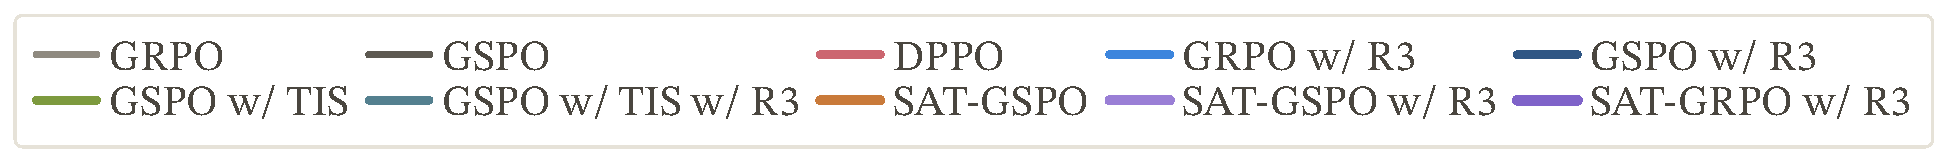
\includegraphics[width=0.85\linewidth]{figures/charts/result_3_4_3_training_mismatch_legend.pdf}
\vspace{-0.2em}

\begin{subfigure}[t]{0.495\linewidth}
\centering
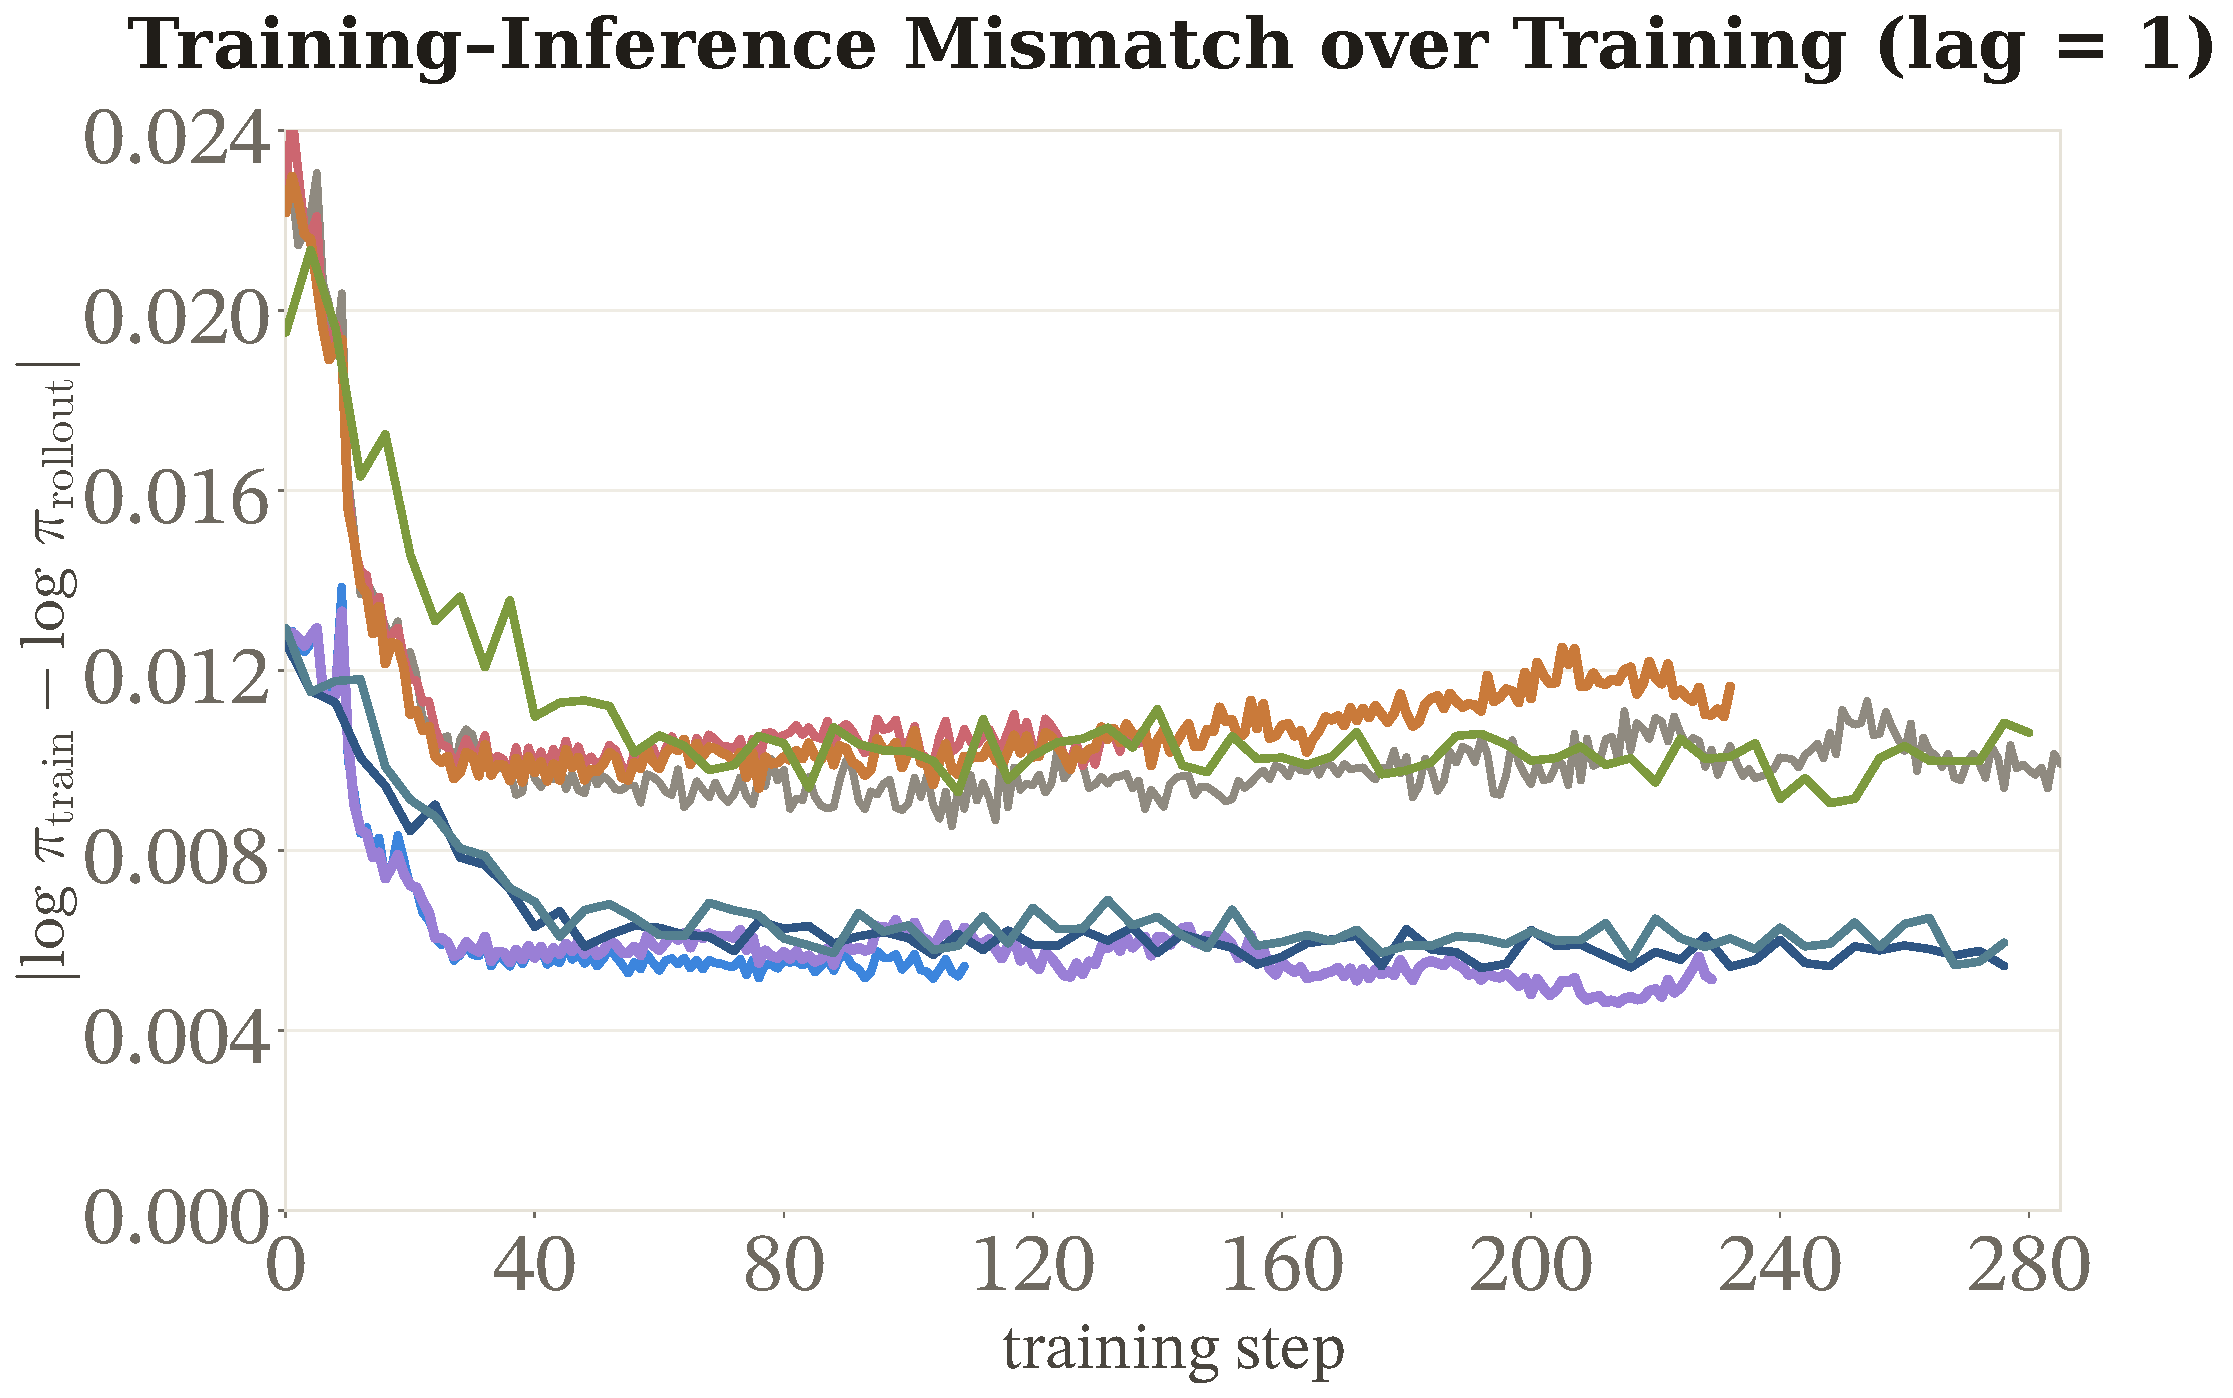
\includegraphics[width=\linewidth]{figures/charts/result_3_4_3a_training_mismatch_lag1.pdf}
\caption{configured lag $=1$}
\label{fig:drift-s1}
\end{subfigure}\hfill
\begin{subfigure}[t]{0.495\linewidth}
\centering
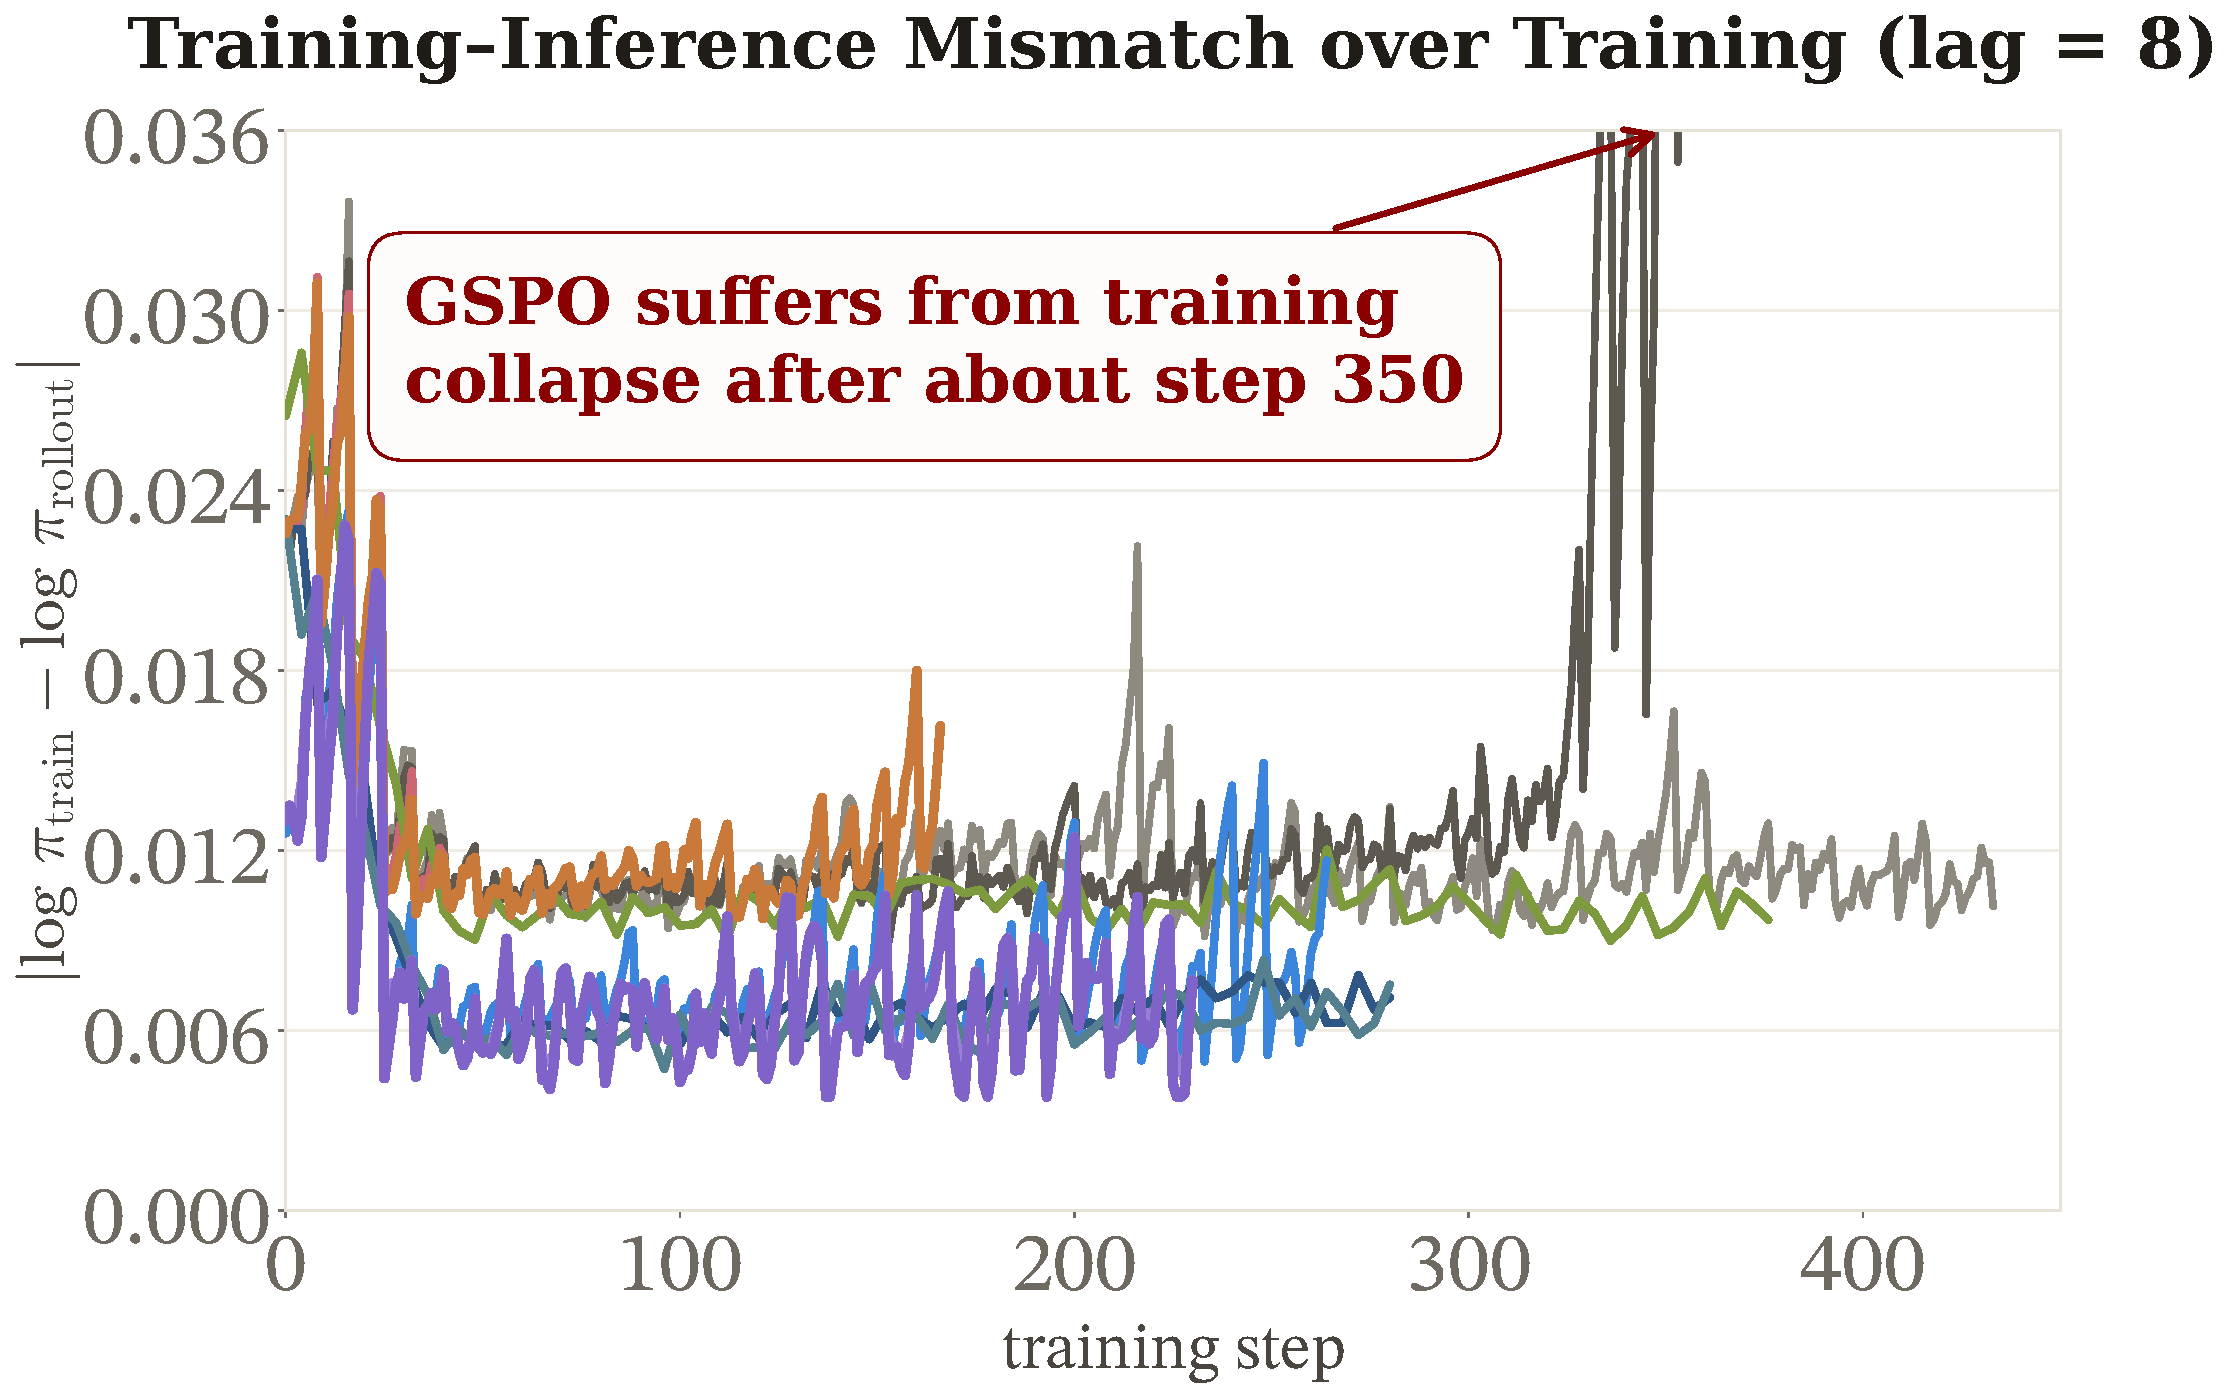
\includegraphics[width=\linewidth]{figures/charts/result_3_4_3b_training_mismatch_lag8.pdf}
\caption{configured lag $=8$}
\label{fig:drift-s8}
\end{subfigure}
\vspace{0.3em}
\caption{\textbf{Training--inference mismatch $\dpi$ over training at configured lag $1$ and $8$.} This figure tracks the batch-averaged sampled mismatch of variance methods across training, with a shared legend distinguishing configurations and separate panels contrasting the mild-lag setting with the high-lag setting.}
\label{fig:drift-pair}
\end{figure}

% Figure~\ref{fig:drift-pair} tracks the mismatch diagnostic behind Table~\ref{tab:main-combined}. Three findings stand out. First, \emph{\satr{} does not buy its results by forcing the logged mismatch to collapse}: at both lags its curves remain close to the corresponding base recipe, which is consistent with the fact that \satr{} acts by reshaping the sampled clip interval rather than by directly redefining the ratio statistic. Second, \emph{routing replay dominates the mismatch level}: the R3-augmented runs occupy the lowest band in both panels, especially in the lag-$8$ setting. Third, the combination explains the complementarity seen in Table~\ref{tab:main-combined}: in these runs, R3 mainly reduces the observed mismatch level, while \satr{} changes where outward gradients stop. The figure is therefore evidence about interaction patterns among stabilizers, not proof of a unique causal ordering between R3 and \satr.
\textbf{Routing replay stabilizes the log prob difference while \satr{} thrives at lower values.} Figure~\ref{fig:drift-pair} tracks the mismatch diagnostic across variance methods behind Table~\ref{tab:main-combined}. 
The integration of routing routing replay (R3) is essential for stabilization: methods utilizing R3 restrict the log prob difference to a tight fluctuation around 0.007. 
Conversely, without R3, the metric deviates noticeably, drifting to around 0.011. 
Second, in the later stages of GRPO training, omitting R3 results in a sudden, sharp growth in the log prob difference. 
Moreover, \textbf{\satr{} achieves better performance while maintaining a lower log prob difference} without training collapse, proving its robustness in managing training dynamics without relying on excessive policy divergence.



\subsection{Asymmetric clipping in \satr{}}
\label{sec:exp-asymclip}

The benchmark table and the mismatch trajectories suggest that the stabilizers differ not only in strength but also in update geometry. A useful organizing principle is the asymmetric clipping family, which includes PPO, DPPO, SPO, DRPO, and \satr{}. For a fixed sampled token with ratio $r_t$ and advantage $\hat A_t$, the unclipped surrogate has derivative $\hat A_t$ with respect to $r_t$, so the sign of $\hat A_t$ determines the locally preferred direction. Relative to $r_t=1$, the sampled update is locally diverging when $\operatorname{sign}(\hat A_t(r_t-1))>0$ and locally converging when $\operatorname{sign}(\hat A_t(r_t-1))<0$. PPO therefore keeps the gate:
\begin{equation}
M_t^{\mathrm{PPO}}
=\mathbf 1\Bigl\{\operatorname{sign}(\hat A_t(r_t-1))\le 0\ \vee\ |r_t-1|\le\varepsilon\Bigr\},
\label{eq:exp-asym-ppo-mask}
\end{equation}
which clips only those updates that would move the sampled ratio farther away from one and preserves the updates that move it back toward the behavior reference.

% DPPO keeps the same directional logic but changes the discriminator. Under the sampled $D_{\mathrm{TV}}$ discriminator:
% \begin{equation}
% D_t^{\mathrm{TV}}
% =\bigl|\pi^{(j)}(y_t\mid s_t)-\mu(y_t\mid s_t)\bigr|
% =\mu(y_t\mid s_t)\,|r_t-1|,
% \label{eq:exp-asym-bintv}
% \end{equation}
% so the condition $D_t^{\mathrm{TV}}\le\delta$ is equivalent to:
% \begin{equation}
% |r_t-1|\le \frac{\delta}{\mu(y_t\mid s_t)}.
% \label{eq:exp-asym-dppo-eps}
% \end{equation}
% The induced gate is:
% \begin{equation}
% M_t^{\mathrm{DPPO}}
% =\mathbf 1\Bigl\{\operatorname{sign}(\hat A_t(r_t-1))\le 0\ \vee\ |r_t-1|\le\delta/\mu(y_t\mid s_t)\Bigr\},
% \label{eq:exp-asym-dppo-mask}
% \end{equation}
% which is tighter on head tokens and looser on long-tail tokens. SPO and DRPO replace the hard gate by quadratic penalties, but the directional structure is the same: outward updates are penalized first, while updates that move the sampled ratio back toward one remain available.

DPPO retains the directional logic but updates the discriminator. The sampled total variation distance $D_t^{\mathrm{TV}}$ bounds the ratio deviation $|r_t-1|$, logically defining the induced gate $M_t^{\mathrm{DPPO}}$:
\begin{equation}
\begin{aligned}
D_t^{\mathrm{TV}} &=\bigl|\pi^{(j)}(y_t\mid s_t)-\mu(y_t\mid s_t)\bigr| =\mu(y_t\mid s_t)\,|r_t-1|, \\
|r_t-1| &\le \frac{\delta}{\mu(y_t\mid s_t)}, \\
M_t^{\mathrm{DPPO}} &=\mathbf 1\Bigl\{\operatorname{sign}(\hat A_t(r_t-1))\le 0\ \vee\ |r_t-1|\le\delta/\mu(y_t\mid s_t)\Bigr\}.
\end{aligned}
\label{eq:dppo_formulation}
\end{equation}

This gating mechanism imposes a more stringent constraint on high-probability head tokens, while granting a more permissive update allowance to rare, low-probability tokens residing in the long tail of the distribution.

% SPO and DRPO substitute quadratic penalties for this hard gate while maintaining the same directional structure.



 The results in Table~\ref{tab:main-combined} and Figure~\ref{fig:asym-dppo-bar} support this view. DPPO reaches $33.96$ at lag $1$ and $32.71$ at lag $8$, outperforming the GRPO baseline at both lags and avoiding the later collapse seen in GRPO and GSPO. This shows that an asymmetric gate with a token-adaptive $D_{\mathrm{TV}}$ threshold can already improve stability in the reported async regime, although DPPO still trails \satr-GSPO at lag $1$ and \satr-GSPO w/ R3 at both lags.


\begin{wrapfigure}{r}{0.5\textwidth}
\vspace{-1.5em}
\centering
\begin{tikzpicture}
\begin{axis}[
width=0.5\textwidth,
height=5cm,
ybar=2pt,
bar width=9.9pt,
ymin=30,
ymax=39,
symbolic x coords={GRPO,GSPO,DPPO,{SAT-GSPO},{SAT-GSPO w/ R3}},
xtick=data,
xticklabel style={font=\fontsize{11.25}{13.5}\selectfont,rotate=25,anchor=east},
yticklabel style={font=\fontsize{7.5}{9}\selectfont},
label style={font=\fontsize{10.5}{12}\selectfont},
legend style={font=\fontsize{11.25}{13.5}\selectfont,draw=none,fill=none,at={(0.5,1.03)},anchor=south,legend columns=2},
ylabel={AIME24 avg@8},
enlarge x limits=0.14,
axis line style={black!35},
tick style={black!35},
nodes near coords,
nodes near coords style={
    font=\fontsize{11.25}{13.5}\selectfont,
    rotate=90,
    anchor=west,
    inner sep=1pt,
    /pgf/number format/fixed,
    /pgf/number format/fixed zerofill,
    /pgf/number format/precision=2
},
every node near coord/.append style={xshift=0pt,yshift=0pt}
]
\addplot+[draw=none,fill=cGRPO] coordinates {(GRPO,31.25) (GSPO,32.25) (DPPO,33.96) ({SAT-GSPO},34.17) ({SAT-GSPO w/ R3},35.83)};
\addplot+[draw=none,fill=cSienna] coordinates {(GRPO,30.17) (GSPO,31.46) (DPPO,32.71) ({SAT-GSPO},32.71) ({SAT-GSPO w/ R3},34.79)};
\legend{lag $=1$, lag $=8$}
\end{axis}
\end{tikzpicture}
\caption{AIME24 avg@8 for GRPO, GSPO, DPPO, and \satr{} variants.}
\label{fig:asym-dppo-bar}
\vspace{-3.5em}
\end{wrapfigure}

Together with Figure~\ref{fig:drift-pair}, the comparison also shows that asymmetry alone is not sufficient: the rule used to set the effective boundary matters. DPPO and \satr{} both preserve pull-back updates and intercept outward ones, but \satr{} chooses the active boundary from the observed mismatch tail of the current batch. Equations~\eqref{eq:satr-clip} and~\eqref{eq:satrloss}, together with Propositions~\ref{prop:containment} and~\ref{prop:pessimism}, formalize this point: \satr{} maintains the asymmetric attribute while cutting off only the newly intercepted outward band. A broader method-by-method comparison is deferred to Appendix~\ref{app:stabilizers} and Appendices~\ref{app:gspo-seqclip}--\ref{app:rollout-lp}.

\FloatBarrier

% Temporarily disabled: Effective clip radii subsection is under revision.
\iffalse
\subsection{Effective clip radii}
\label{sec:exp-radius}

\begin{figure}[htbp]
\centering
\begin{tikzpicture}
\begin{axis}[width=0.62\textwidth,height=5.4cm,
  xlabel={training step},ylabel={effective clip radius (mean on active tokens)},
  label style={font=\scriptsize},tick label style={font=\tiny},
  xmin=0,xmax=205,ymin=0,ymax=0.02,
  ytick={0,0.005,0.01,0.015,0.02},
  legend style={font=\scriptsize,draw=none,fill=none,at={(0.03,0.97)},anchor=north west},
  every axis plot/.append style={line width=0.7pt}]
\addplot[name path=lolo,draw=none,forget plot] table[y=ylo] {figures/data/eps_low_band.dat};
\addplot[name path=lohi,draw=none,forget plot] table[y=yhi] {figures/data/eps_low_band.dat};
\addplot[cAccent!30,forget plot] fill between[of=lolo and lohi];
\addplot[name path=hilo,draw=none,forget plot] table[y=ylo] {figures/data/eps_high_band.dat};
\addplot[name path=hihi,draw=none,forget plot] table[y=yhi] {figures/data/eps_high_band.dat};
\addplot[cSienna!30,forget plot] fill between[of=hilo and hihi];
\addplot[cAccent] table {figures/data/eps_low_mean.dat};
\addlegendentry{$\bar\varepsilon_{\mathrm{low}}$ (mean $\pm 1\sigma$)}
\addplot[cSienna] table {figures/data/eps_high_mean.dat};
\addlegendentry{$\bar\varepsilon_{\mathrm{high}}$ (mean $\pm 1\sigma$)}
\end{axis}
\end{tikzpicture}
\caption{\textbf{\satr{} effective clip radii over training.} Cross-run mean $\pm 1\sigma$ of the per-step means $\bar\varepsilon_{\mathrm{low}}$ and $\bar\varepsilon_{\mathrm{high}}$ across 14 \satr{} runs. The upper radius remains above the lower radius in the reported runs.}
\label{fig:eps}
\end{figure}

Figure~\ref{fig:eps} aggregates the radii \satr{} emits at every optimizer step through Equations~\eqref{eq:gate}--\eqref{eq:adaptive-eps}. Two cautions govern the reading. The raw means combine two effects---the base radii and the sign distribution of gated mismatches---so they should be interpreted together with the normalized factors $\E[c_-]$, $\E[c_+]$, the realized gate rate, and $q$ (Appendix~\ref{app:monitor}). And while a crossing of the two raw means ($\bar\varepsilon_{\mathrm{low}}>\bar\varepsilon_{\mathrm{high}}$) is a useful diagnostic that the gated mismatch has shifted to the negative side, such a crossing neither proves a universal positive drift nor, by itself, determines that the quantile hyper-parameter should be changed. In the reported runs the asymmetry persists and no reversal occurs, consistent with their stable training curves.

\FloatBarrier
\fi

% =====================================================================
% 6 Limitations and open questions
% =====================================================================
\section{Open Questions}
\label{sec:limitations}

% The current scope is intentionally narrow, and the main limitations are:
While the current experimental scope only focusing the setting of reinforcement learning for improving LLM's reasoning capability, the underlying SAT methodology demonstrates strong potential for broader application across diverse learning domains, leaving main limitations as follows:
\begin{itemize}
\item \textbf{Surrogate-level control.} \satr{} contracts a sampled nominal interval rather than the realized policy itself. The learned policy can still move outside that interval, unobserved vocabulary actions remain unconstrained, and the proxy $|\log r|$ should not be identified with either $D_{\mathrm{TV}}$ or version age because it omits the probability-mass weight in Equation~\eqref{eq:tv-mass} and mixes policy lag with implementation mismatch.
\item \textbf{Relative adaptation.} Because the reference quantile $q$ is recomputed for every batch, the method responds to the current mismatch tail rather than to an absolute scale. It therefore does not imply monotone shrinkage with configured lag once PPO's original boundary is already active.
\end{itemize}

% =====================================================================
% 7 Conclusion
% =====================================================================
\section{Conclusion}
\label{sec:conclusion}

The trust-region interpretation of \satr{} is narrow but clear. $D_{\mathrm{TV}}$ controls a finite-horizon approximation term, and $D_{\mathrm{TV}}$ is exactly a behavior expectation of absolute ratio deviation, so a hard all-action ratio bound would control $D_{\mathrm{TV}}$. PPO does not impose such a bound and instead clips an advantage-dependent sampled surrogate. \satr{} operates at that same surrogate level by using a detached mismatch proxy to contract the sign-selected nominal radius on the high-staleness tail of each batch. Its effect is therefore local but precise: it cuts off newly intercepted outward updates earlier while preserving pull-back gradients, and it reduces exactly to the underlying recipe when disabled. On the reported grid, \satr-GSPO w/ R3 attains the best-observed AIME24 avg@8 at both configured lags, reaches $35.83$ at lag $1$ and $34.79$ at lag $8$, and avoids the late collapse seen in several fixed-clip lag-$8$ baselines. Together with the interval-containment and pointwise-pessimism results, these findings give a concrete account of what an adaptive $\varepsilon$ can contribute in asynchronous RL.
